% This is my template for presentations of diploma
% All slides in code separated by line

\documentclass[ucs,compress]{beamer}    % [ucs] makes Cyrillic fonts visible in index 
\usepackage{beamerthemeshadow} % use <beamerthemeshadow> theme
\usepackage[T2A]{fontenc}
\usepackage[utf8]{inputenc}    % set encoding
\usepackage[english,ukrainian]{babel}
\usepackage{amssymb,amsfonts,amsmath}
\usepackage{cite,enumerate,float,indentfirst}
\usepackage{graphicx,epstopdf}    % epstopdf-convert eps files to pdf
\graphicspath{{fig/},{software/}} % look up folders for figures

\usepackage{color}     % you can colour your formulas with this, just use ${\color{red} E=mc^2}$
\usepackage{helvet} 	       % set font family for whole document
\usefonttheme[onlymath]{serif} % Set font family only for math mode

% \beamertemplatenavigationsymbolsempty

% If you want divide slide on two parts just use code:
% \begin{columns}[t]
% \begin{column}{5cm}
%  some data in column 1
% \end{column}
% \begin{column}{5cm}
%  some data in column 2
% \end{column}
% \end{columns}

% If you want to make theorem or emphasize some info, use next code:
% \begin{block}{title of block}
% Some data in block, feel free to add formulas,tables or figures here.
% \end{block} 

% use \begin{frame}[shrink=5] in case if you need insert more text in slide

\begin{document}
\title{Інтегрована інерціально-супутникова система навігації, що базується на принципах комплексної обробки інформації
з використанням калманівської фільтрації}  
% \author{доповідач:Микола Новік\\ керівник: Мар’ясова Т.І.}
\author{Микола Новік}
\date{\today} 
%%%%<<<<<<<<<<<<<<<<<<<<<<<<<<<<<<<<<<<<<<<<<<<<<<<<<<<<<<<<<<<<<<<<<<<<<<<<<<<<<<<
% First Slide, title page
\begin{frame}
\titlepage
\end{frame}
%%%%<<<<<<<<<<<<<<<<<<<<<<<<<<<<<<<<<<<<<<<<<<<<<<<<<<<<<<<<<<<<<<<<<<<<<<<<<<<<<<<
% Just print table of contents
\begin{frame}[plain]
\frametitle{Зміст доповіді}
\tiny
\tableofcontents
\end{frame} 
%%%%<<<<<<<<<<<<<<<<<<<<<<<<<<<<<<<<<<<<<<<<<<<<<<<<<<<<<<<<<<<<<<<<<<<<<<<<<<<<<<<
% Intro
\section{Постановка задачі та вибір системи} 
\subsection{Постановка задачі та вибір системи} 
\begin{frame}\frametitle{Постановка задачі комплексування}
\small
\beamerbutton{\smallПостановка задачі}: дослідження можливостей комплексування навігаційної інформації двох систем, що є на борту сучасного літака: безплатформенної інерціальної навігаційної системи і супутникової високоточної навігаційної системи.\\
\centering \line(1,0){200}

\begin{block}<+->{В результатi комплексування IНС та СНС досягаються:}
\tiny
\begin{enumerate}
\item  пiдвищення точностi визначення координат, висоти, швидкостi i часу споживача;
\item  уточнення кутiв орiєнтацiї (курсу, крену i тангажа);
\item  оцiнка й уточнення параметрiв калiбрування навiгацiйних датчикiв,
таких, як дрейфи гiроскопiв, масштабнi коефiцiєнти, зсуви акселерометрiв тощо;
\item  забезпечення на цiй основi безперервностi навiгацiйних визначень на всiх етапах руху, у тому числi i при тимчасовiй непрацездатностi приймача СНС у випадках впливу завад або енергiйних маневрiв ЛА.

\end{enumerate}
\end{block}

\end{frame} 

%%%%<<<<<<<<<<<<<<<<<<<<<<<<<<<<<<<<<<<<<<<<<<<<<<<<<<<<<<<<<<<<<<<<<<<<<<<<<<<<<<<
\subsection{Вибір варіанту комплексування ІСНС } 
\begin{frame}\frametitle{Варіанти інтегрування ІСНС} 

\tiny
\begin{block}{Роздільна}
Надмірність, обмеженість похибок оцінок місця розташування і швидкості, 
наявність інформації про орієнтацію і кутову швидкість, висока швидкість видачі інформації, 
мінімальні зміни в бортовій апаратурі
\end{block}

\begin{exampleblock}{Слабко зв'язана}
Усі перераховані особливості роздільних систем, плюс більш 
швидке відновлення слідкування за кодом і фазою сигналів СНС, виставлення та калібрування 
БІНС у польоті, як наслідок -- підвищена точність під час відсутності сигналу СНС
\end{exampleblock}


\begin{block}{Жорстко зв'язана}
Подальше поліпшення точності і калібрування, підвищена стійкість слідкування 
за сигналами СНС при маневрах ЛА, підвищена завадостійкість 
\end{block}

\begin{block}{Глибоко інтегрована}
Єдиний фільтр усуває проблему ``каскадного'' включення 
фільтрів, компактність, знижені вимоги з енергозабезпечення. Недоліки: вектор стану 
містить до 40 компонентів, тому фільтр складно реалізувати; необхідність розробки 
спеціальних датчиків 
\end{block}
\end{frame}
%%%%<<<<<<<<<<<<<<<<<<<<<<<<<<<<<<<<<<<<<<<<<<<<<<<<<<<<<<<<<<<<<<<<<<<<<<<<<<<<<<<


\subsection{Схема комплексування ІСНС }
\begin{frame} \frametitle{Схема ІСНС} 
\begin{figure}[here]
\centering
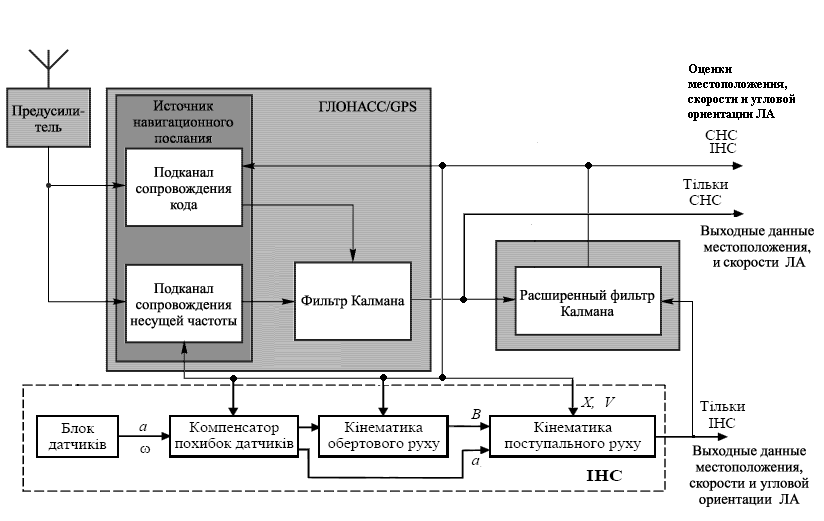
\includegraphics[width=90mm,height=65mm]{structure_scheme2}
\caption{Слабко зв’язана схема}
%\label{fig:isns_loosly}
\end{figure}
\end{frame}
%%%%<<<<<<<<<<<<<<<<<<<<<<<<<<<<<<<<<<<<<<<<<<<<<<<<<<<<<<<<<<<<<<<<<<<<<<<<<<<<<<<

\section{Модель системи }

\subsection{Алгоритми роботи БІНС} 
\begin{frame}[plain]
\frametitle{Алгоритми роботи БІНС}
\tiny
\begin{columns}[t]
\begin{column}{5cm}
\beamerbutton{Швидкий темп}
$\label{eq:fgyro} 
\begin{array}{l} 
{\omega_{y_{\Sigma }} =\omega_{y_{\text{ЛА}}} -\omega_{y_{NHE}};} \\ 
{\omega_{x_{\Sigma }} =\omega_{x_{\text{ЛА}}} -\omega_{x_{NHE}};} \\ 
{\omega_{z_{\Sigma }} =\omega_{z_{\text{ЛА}}} -\omega_{z_{NHE}}.} 
\end{array}$
\vspace{3mm}
$\label{eq:fangle} 
\begin{array}{l} 
{\dot{\psi }=(\omega_{y_{\Sigma }}\cos \gamma -\omega_{z_{\Sigma }} \sin \gamma)\sec \vartheta ;} \\ 
{\dot{\gamma }=\omega_{x_{\Sigma}} +{\rm tg}\vartheta {\rm \; }\left(\omega_{z_{\Sigma}} \sin \gamma -\omega_{y_{\Sigma}} \cos \gamma \right);} \\ 
{\dot{\vartheta }=\omega_{y_{\Sigma}}\sin \gamma +\omega_{z_{\Sigma }} \cos \gamma;} \\ 
{\psi_{\text{г}} =-\psi .} \end{array} 
$

\beamerbutton{Середній темп}
$\label{eq:maccel} 
\left[\begin{array}{c} 
{a_{N}} \\ 
{a_{H}} \\ 
{a_{E}} \end{array}\right]=
B\left[\begin{array}{c} 
{a_{x_{\text{ЛА}}}} \\ 
{a_{y_{\text{ЛА}}}} \\ 
{a_{z_{\text{ЛА}}}} 
\end{array}\right]$
\vspace{3mm}
$\label{eq:mdv} 
\begin{array}{l} 
{\dot{V}_{E} =a_{E} -V_{N}(\omega_{H_{V}} +2\Omega_{H} )+V_{H} (\omega_{N_{V}} +2\Omega_{N} );} \\ 
{\dot{V}_{H} =a_{H} -V_{E}(\omega_{N_{V}} +2\Omega_{N} )+V_{N} \omega_{E_{V}} +g_{H} ;} \\ 
{\dot{V}_{N} =a_{N} -V_{H} \omega_{E_{V}} +V_{E} (\omega_{H_{V}} +2\Omega_{H} ).} 
\end{array} 
$
\end{column}

\begin{column}{5cm}
\beamerbutton{Повільний темп}

$\label{eq:geocord} 
\begin{array}{l} 
{\dot{\lambda}=\frac{V_{E}}{(R_{2}+H)\cos B};} \\ 
{\dot{\varphi}=\frac{V_{N}}{R_{1}+H} ;} \\ 
{\dot{H}=V_{H}.} 
\end{array} $
\vspace{3mm}
$\label{eq:__8_26_} 
\begin{array}{l} 
{\omega_{E_{V}} =-\dot{\varphi};} \\ 
{\omega_{H_{V}} =\dot{\lambda}{sin}\varphi;} \\ 
{\omega_{N_{V}} =\dot{\lambda}\cos \varphi;} \\ 
{\Omega_{N} =\Omega_{\text{З}}\cos \varphi;} \\ 
{\Omega_{H} =\Omega_{\text{З}}\sin \varphi.} 
\end{array} $ 
\vspace{3mm}
$\label{eq:lomega}
\left[\begin{array}{c} 
{\omega_{x_{NHE}}} \\ 
{\omega_{y_{NHE}}} \\ 
{\omega_{z_{NHE}}} \end{array}\right]=B^{T} 
\left[\begin{array}{c} 
{\omega_{N_{V}} +\Omega_{N}} \\ 
{\omega_{H_{V}} +\Omega_{H}} \\ 
{\omega_{E_{V}} +\Omega_{E}} 
\end{array}\right].$
 
\end{column}
\end{columns}

{\centering \line(1,0){300}\\}
де: \\
$\label{eq:bmatrix}
B=\left[\begin{array}{ccc} 
{\cos \psi \cos \vartheta } & 
{\sin \psi \sin \gamma -\cos \psi \sin \vartheta \cos \gamma } & 
{\sin \psi \cos \gamma +\sin \psi \cos \vartheta \sin \gamma } \\ 
{\sin \vartheta } & {\cos \vartheta \cos \gamma } & 
{-\cos \vartheta \sin \gamma } \\ 
{-\sin \psi \cos \vartheta } & 
{\cos \psi \sin \gamma +\sin \psi \sin \vartheta \cos \gamma } & 
{\cos \psi \cos \gamma -\sin \psi\sin \vartheta \sin \gamma } 
\end{array}\right]. 
$\\
\vspace{3mm}
$\label{eq:gravity} 
\begin{array}{l}{\frac{1}{(R_{1} +H)} \approx \frac{1}{a}\left[1-e^{2} -\frac{H}{a} -\frac{3}{2} e^{2} \sin ^{2} \varphi\right];} \\ 
{\frac{1}{(R_{2} +H)} \approx \frac{1}{a} \left[1-\frac{H}{a} -\frac{1}{2} e^{2} \sin ^{2}\varphi\right]  ;} \\ 
{g_{H} =-g\left(1+5,2884\cdot 10^{-3} \sin ^{2}\varphi \right)\left[1-\frac{2H}{a} \left(1-e\sin ^{2}\varphi \right)\right].} 
\end{array}$
\end{frame}

%%%%<<<<<<<<<<<<<<<<<<<<<<<<<<<<<<<<<<<<<<<<<<<<<<<<<<<<<<<<<<<<<<<<<<<<<<<<<<<<<<<
\subsection{Рівняння похибок БІНС} 
\begin{frame}[plain]
\frametitle{Рівняння похибок БІНС}
\begin{block}{БІНС}
\tiny
Похибка приведеної координати:\\
$\begin{array}{l} 
{\Delta \dot{R}_{E} =\Delta V_{E}(t)\cdot \frac{R_{\text{З}} }{R\cos \varphi (t)} 
+\Delta R_{N} (t)\frac{V_{E}^{}(t)\sin \varphi (t)}{R_{\text{З}} R\cos ^{2} \varphi (t)} 
-\Delta h(t)\frac{R_{\text{З}} V_{E}^{}(t)}{R^{2} \cos \varphi (t)} ;} \\ 
{\Delta \dot{R}_{N} =\Delta V_{N}(t)\cdot \frac{R_{\text{З}}}{R} -\Delta h(t)\frac{R_{\text{З}} V_{N}(t)}{R^{2}};} \\ 
{\Delta \dot{h} =\Delta V_{h} (t);} \end{array} $

{\centering \line(1,0){300}\\}
Похибка швидкості:\\
$\begin{array}{l}{\Delta \dot{V}_{E} =a_{N} \alpha_{h} -a_{h} \alpha_{N} +\sum_{i=1}^{3}b_{1,i}  \Delta a_{i} -\Delta V_{h} U(t)\cos \varphi +\Delta V_{N}U(t)\sin \varphi +} \\ 
{+\frac{\Delta R_{N} }{R_{\text{З}} } \left(U(t)(V_{h} \sin \varphi +V_{N}\cos \varphi \right))-(\frac{\Delta V_{E} }{R\cos \varphi } +\frac{V_{E} \sin \varphi}{R\cos ^{2} \varphi } \frac{\Delta R_{N} }{R_{\text{З}} } )\times } \\ 
{\times (V_{h} \cos \varphi -V_{N} \sin \varphi )+\frac{\Delta hV_{E} }{R^{2} } (V_{h} -V_{N}tg\varphi);} \\
\\
{\Delta \dot{V}_{N} =-a_{E}\alpha_{h} +a_{h} \alpha_{E} +\sum_{i=1}^{3}b_{2,i}  \Delta a_{i} -\Delta V_{E}U(t)\sin \varphi -\Delta V_{h} \dot{\varphi }(t)-} \\ 
{-\frac{\Delta R_{N} }{R_{\text{З}}} V_{E} U(t)\cos \varphi -\frac{\Delta V_{N} }{R} V_{h} -(\frac{\Delta V_{E} }{R\cos \varphi } +\frac{V_{E} \sin \varphi }{R\cos ^{2} \varphi } \frac{\Delta R_{N} }{R_{\text{З}} } )V_{E} \sin \varphi +} \\ 
{+\frac{\Delta h}{R^{2} } (V_{E}^{2} tg\varphi +V_{N} V_{h} );} \\
\\
{\Delta \dot{V}_{h} =a_{E} \alpha_{N} -a_{N} \alpha_{E} +\sum_{i=1}^{3}b_{3,i}  \Delta a_{i} +\Delta V_{E} U(t)\cos \varphi +\Delta V_{N} \dot{\varphi }(t)-} \\ 
{-\frac{\Delta R_{N} }{R_{\text{З}} } V_{E} U(t)\sin \varphi +\frac{\Delta V_{N} }{R} V_{N} +(\frac{\Delta V_{E} }{R\cos \varphi } +\frac{V_{E} \sin \varphi }{R\cos ^{2} \varphi } \frac{\Delta R_{N} }{R_{\text{З}} } )V_{E} \cos \varphi +} \\ 
{+g_{e} \left(-\frac{2\Delta h}{a} +\frac{3}{2} e^{2} \sin \varphi \cos \varphi \frac{\Delta R_{N} }{R_{\text{З}} } \right)-\frac{\Delta h}{R^{2} } \left(V_{E}^{2} +V_{N}^{2} \right),} 
\end{array}\label{eq:dVsdins}$

{\centering \line(1,0){300}\\}
Похибка координатного тригранника:\\
$\label{eq:dasdins} \begin{array}{l} 
{\dot{\alpha }_{E} =-\omega_{N} \alpha_{h} +\omega_{h} \alpha_{N} -\frac{\Delta V_{N} }{R} -\sum_{i=1}^{3}b_{1,i}\varepsilon_{i} ,} \\
{\dot{\alpha }_{N} =-\omega_{h} \alpha_{E} +\omega_{E} \alpha_{h} +\frac{\Delta V_{E} }{R} -u\sin \varphi \frac{\Delta R_{N} }{R_{7} }
-\sum_{i=1}^{3}b_{2,i}  \varepsilon_{i} ,} \\ 
{\dot{\alpha }_{h} =-\omega_{E} \alpha_{N} +\omega_{N} \alpha_{E} +\frac{\Delta V_{E} }{R} tg\varphi +(u\cos \varphi +\frac{V_{E} }{R\cos ^{2} \varphi } )
\frac{\Delta R_{N} }{R_{7} } -\sum_{i=1}^{3}b_{3,i}\varepsilon_{i} ,} \end{array} $
\end{block}
\end{frame}

%%%%<<<<<<<<<<<<<<<<<<<<<<<<<<<<<<<<<<<<<<<<<<<<<<<<<<<<<<<<<<<<<<<<<<<<<<<<<<<<<<<
\subsection{Матриця динаміки БІНС} 
\begin{frame}[plain,shrink=10]
\frametitle{Матриця динаміки БІНС}
\small
% F_{p,k}
\[F_{p,k} = \left(\begin{array}{cccc cc}
% {1} & {2} & {3} & {4} & {5} & {6} & {7} & {8} & {9} & {0} & {1} & {2} & {3} & {4} & {5}\\ 
% Position
{.} & {\frac{\dot{\lambda }}{R_{\text{З}} } tg\varphi;} & {\frac{-\dot{\lambda }R_{\text{З}} }{R}} & {\frac{R_{\text{З}} }{R\cos \varphi }} & {.} & {.} \\
{.} & {.} & {\frac{-\dot{\varphi }R_{\text{З}} }{R}} & {.} & {\frac{R_{\text{З}} }{R}} & {.} \\
{.} & {.} & {.} & {.} & {.} & {1} \\
% Velocity
{.} & {\begin{array}{c}{\frac{2u+\dot{\lambda }}{R_{\text{З}} } \left(V_{h} \sin \varphi  +V_{N} \cos \varphi \right)}\\
{-\frac{\dot{\lambda }}{R_{\text{З}} } tg\varphi \left(V_{h} \cos \varphi -V_{N} \sin \varphi \right)}\end{array}} & 
{\frac{V_{E} }{R^{2} } \left(V_{h} -V_{N} tg\varphi \right)} & 
{\frac{V_{N}\sin \varphi -V_{h} \cos \varphi }{R\cos \varphi }} & 
{\left(2u+\dot{\lambda }\right)\sin \varphi} & 
{-\left(2u+\dot{\lambda }\right)\cos \varphi} \\ 

{.} & {-\frac{2u+\dot{\lambda }}{R_{\text{З}} }V_{E} \cos \varphi -\frac{V_{E}^{2} }{RR_{\text{З}} } tg^{2} \varphi} & 
{\frac{V_{E}^{2} tg\varphi +V_{h} V_{N} }{R^{2} }} & 
{-\left(2u+\dot{\lambda }\right)\sin \varphi;} & 
{-\frac{V_{h} }{R}} & 
{-\dot{\varphi }(t)} \\ 

{.} & {-2u\frac{V_{E}^{} \sin \varphi }{R} +\frac{3g_{e} }{2R_{\text{З}}} e^{2} \sin \varphi \cos \varphi} & 
{-\frac{2g_{e} }{a} -\frac{V_{E}^{2} +V_{N}^{2}}{R^{2}}} & 
{\left(2u+\dot{\lambda }\right)\cos \varphi} & 
{\dot{\varphi }(t)+\frac{V_{N} }{R}} & {.} \\
 

% Alpha
{.} & {.} & {.} & {.} & {-\frac{1}{R}} & {.} \\ 
{.} & {-\frac{u}{R} \sin \varphi} & {.} & {\frac{1}{R}} & {.} & {.} \\ 
{.} & {\frac{1}{R}_{7} (u\cos \varphi +\frac{\dot{\lambda }}{\cos \varphi })} & {.} & {\frac{tg\varphi }{R}} & {.} & {.} \\ 

% othe staff
{.} & {.} & {.} & {.} & {.} & {.} \\
{.} & {.} & {.} & {.} & {.} & {.} \\
{.} & {.} & {.} & {.} & {.} & {.} \\ 
{.} & {.} & {.} & {.} & {.} & {.} \\
{.} & {.} & {.} & {.} & {.} & {.} \\
{.} & {.} & {.} & {.} & {.} & {.} \\
\end{array}\right. \] 


\[\left. \begin{array}{cccc cccc cccc cc}
% {1} & {2} & {3} & {4} & {5} & {6} & {7} & {8} & {9} & {0} & {1} & {2} & {3} & {4} & {5}\\ 
% Position
{.} & {.} & {.} & {.} & {.} & {.} & {.} & {.} & {.}\\ 
{.} & {.} & {.} & {.} & {.} & {.} & {.} & {.} & {.}\\ 
{.} & {.} & {.} & {.} & {.} & {.} & {.} & {.} & {.}\\ 

{.} & {-a_{h}} & {a_{N}} & {.} & {.} & {.} & 
{b_{1,1}} & {b_{1,2}} & {b_{1,3}}\\ 

{a_{h}} & {.} & {-a_{E}} & {.} & {.} & {.} & 
{b_{2,1}} & {b_{2,2}} & {b_{2,3}}\\ 

{-a_{N}} & {a_{E}} & {.} & {.} & {.} & {.} & 
{b_{3,1}} & {b_{3,2}} & {b_{3,3}}\\

{.} & {\omega_{h}} & {-\omega_{N}} & 
{-b_{1,1}} & {-b_{1,2}} & {-b_{1,3}} & {.} & {.} & {.}\\

{-\omega_{h}} & {.} &{\omega_{E}} & 
{-b_{2,1}} & {-b_{2,2}} & {-b_{2,3}} & {.} & {.} & {.}\\

{\omega_{N}} & {-\omega_{E}} & {.} & {-b_{3,1}} & 
{-b_{3,2}} & {-b_{3,3}} & {.} & {.} & {.}\\


{.} & {.} & {.} & {.} & {.} & {.} & {.} & {.} & {.}\\ 
{.} & {.} & {.} & {.} & {.} & {.} & {.} & {.} & {.}\\ 
{.} & {.} & {.} & {.} & {.} & {.} & {.} & {.} & {.}\\

{.} & {.} & {.} & {.} & {.} & {.} & {.} & {.} & {.}\\
{.} & {.} & {.} & {.} & {.} & {.} & {.} & {.} & {.}\\
{.} & {.} & {.} & {.} & {.} & {.} & {.} & {.} & {.}\\ 
\end{array}\right);\] 

\end{frame}

%%%%<<<<<<<<<<<<<<<<<<<<<<<<<<<<<<<<<<<<<<<<<<<<<<<<<<<<<<<<<<<<<<<<<<<<<<<<<<<<<<<
\subsection{Рівняння похибок СНС та БВ} 
\begin{frame}[plain]
\frametitle{Рівняння похибок СНС та БВ}
\tiny
\begin{block}{СНС}
Помилки СНС:\\
$\begin{array}{l} 
{\Delta R_{Es,k} =\Delta R_{Ec,k} +\frac{\sigma_{Rs} }{\cos \varphi_{k} } \eta_{REs,k} +\frac{\sigma_{\delta Rs} }{\cos \varphi_{k} } \eta_{\delta RE,k} ;} \\ 
{\Delta R_{Ns,k} =\Delta R_{Nc,k} +\sigma_{Rs} \eta_{RNs,k} +\sigma_{\delta Rs} \eta_{\delta RN,k} ;} \\ 
{\Delta H_{s,k} =\Delta H_{c,k} +\sigma_{Hs} \eta_{Hs,k} +\sigma_{\delta Rs} \eta_{\delta H,k} }\\ 
{\Delta V_{ls,k} =\Delta V_{lc,k} +\sigma_{Vs} \eta_{V\, ls,k} +\sigma_{\delta Vs} \eta_{\delta V\, ls,k}, \text{при } l=E,N,H;} 
\end{array}$\\
Корельовані помилки СНС:\\
$\begin{array}{l} 
{\Delta R_{Ec,k}=W_{R} \Delta R_{Ec,k-1} +q_{R} \frac{\sigma_{Rc} }{\cos \varphi_{k} } \eta_{REc,k} +\frac{\sigma_{\delta RC} }{\cos \varphi_{k} } \eta_{\delta REc,k} ;} \\ 
{\Delta R_{Nc,k}=W_{R} \Delta R_{Nc,k-1} +q_{R} \sigma_{Rc} \eta_{RNc,k} +\sigma_{\delta RC} \eta_{\delta RNc,k} ;} \\ 
{\Delta H_{c,k}=W_{R}  \Delta H_{c,k-1}  +q_{R} \sigma_{Hc} \eta_{Hc,k} +\sigma_{\delta Hc} \eta_{\delta Hc,k} ;} \\ 
{\Delta V_{lc,k} =W_{V} \Delta V_{lc,k-1} +q_{V}\sigma_{Vc} \eta_{V lc,k} +\sigma_{\delta Vc} \eta_{\delta V lc,k}, \text{при } l=E,N,H,} 
\end{array} $\\
де:
$\begin{array}{l}
{W_{R} =e^{-(\lambda_{s} V_{\text{Ш}} +\lambda_{st} )\Delta t} ; }
{q_{R} =\left[1-\exp \left(-2\left(\lambda_{s} V_{\text{Ш}} +\lambda_{st} \right)\Delta t\right)\right]^{0,5};}\\
{W_{V} =e^{-\lambda_{V} \Delta t};}
{q_{V} =\left[1-\exp \left(-2 \lambda_{V} \Delta t\right)\right]^{0,5};}

\end{array}$\\
Матриця динаміки корельованих поихибок СНС:
$F_{sns} =\left(\begin{array}{cccccccc} 
{W_{R}} & {.} & {.} & {.} & {.} & {.} \\ 
{.} & {W_{R} } & {.} & {.} & {.} & {.} \\ 
{.} & {.} & {W_{R} } & {.} & {.} & {.} \\ 
{.} & {.} & {.} & {W_{V} } & {.} & {.} \\ 
{.} & {.} & {.} & {.} & {W_{V} } & {.} \\ 
{.} & {.} & {.} & {.} & {.} & {W_{V} } 
\end{array}\right) 
$
\end{block}

\begin{block}{БВ}
Дискретна модель похибок БВ:\\
$\Delta h_{c,k} =\Delta h_{c,k-1} +\sigma_{\xi A} \xi_{k-1}$
\end{block}
\end{frame}
%%%%<<<<<<<<<<<<<<<<<<<<<<<<<<<<<<<<<<<<<<<<<<<<<<<<<<<<<<<<<<<<<<<<<<<<<<<<<<<<<<<
\subsection{Рівняння ІНСН в просторі станів}
\begin{frame}[shrink=5] \frametitle{Система в просторі станів} 

\begin{columns}[t]
\begin{column}{5cm}
\noindent 
Вектор стану системи
\begin{equation*}
\tiny
% \bar{X}= 
\left[ \begin{array}{l}
{{\color{blue}\Delta R_{E}}}\\
{{\color{blue}\Delta R_{N}}}\\
{{\color{blue}\Delta h}}\\
{{\color{blue}\Delta V_{E}}}\\
{{\color{blue}\Delta V_{N}}}\\
{{\color{blue}\Delta V_{h}}}\\
{{\color{blue}\alpha_{E}}}\\
{{\color{blue}\alpha_{N}}}\\
{{\color{blue}\alpha_{h}}}\\
{{\color{blue}\varepsilon_{c1}}}\\
{{\color{blue}\varepsilon_{c2}}}\\
{{\color{blue}\varepsilon_{c3}}}\\
{{\color{blue}\Delta a_{c1}}} \\
{{\color{blue}\Delta a_{c2}}}\\
{{\color{blue}\Delta a_{c3}}}\\
{{\color{red}\Delta h_{\text{БВ}}}}\\
{{\color{violet}\Delta R_{Ec}}}\\
{{\color{violet}\Delta R_{Nc}}}\\
{{\color{violet}\Delta h_{c}}}\\
{{\color{violet}\Delta V_{Ec}}}\\
{{\color{violet}\Delta V_{Nc}}}\\
{{\color{violet}\Delta V_{hc}}}
\end{array} \right]=
\left[\begin{array}{l}
{\text{Пом. координ. E}}\\
{\text{Пом. координ. N}}\\
{\text{Пом. по висоті}}\\
{\text{Пом. по швидкості E}}\\
{\text{Пом. по швидкості N}}\\
{\text{Пом. по швидкості H}}\\
{\text{Пом. тригранника E}}\\
{\text{Пом. тригранника N}}\\
{\text{Пом. тригранника H}}\\
{\text{Дрейф гіроскопа E}}\\
{\text{Дрейф гіроскопа N}}\\
{\text{Дрейф гіроскопа H}}\\
{\text{Дрейф акселерометра E}} \\
{\text{Дрейф акселерометра N}}\\
{\text{Дрейф акселерометра H}}\\
{\text{Пом. баровисотоміра}}\\
{\text{Кор. пом. коорд. СНС E}}\\
{\text{Кор. пом. коорд. СНС N}}\\
{\text{Кор. пом. коорд. СНС H}}\\
{\text{Кор. пом. швид. СНС E}}\\
{\text{Кор. пом. швид. СНС N}}\\
{\text{Кор. пом. швид. СНС H}}\\
\end{array} \right]  
\end{equation*}

\end{column}
\begin{column}{5cm}
Моедель системи в просторі станів.\\

\tiny

$\bar{X}_{p,k+1} =\Phi_{p,k} \bar{X}_{p,k} +G_{p,k} \bar{\xi }_{k}$ \\
Матриця динаміки системи\\
$ F_{p,k} =\left(\begin{array}{ccc} 
{F_{k} } & {.} & {.} \\
{.} & {F_{bv}} & {.} \\
{.} & {.} & {F_{sns}} \\
\end{array}\right);$
Коваріаційна матриця шумів\\
$Q_{p,k} =\left(\begin{array}{ccc} 
{Q_{k} } & {.} & {.} \\ 
{.} & {\sigma_{\text{БВ}} \sqrt{\Delta t}} & {.} \\ 
{.} & {.} & {G_{s,k} } \end{array}\right);$
Вимірювання\\
$\bar{Y}_{k} = 
\left(\begin{array}{l}
{\tilde{h}_{k} -\tilde{h}_{\text{БВ},k},}\\
{\tilde{R}_{E,K} -\tilde{R}_{ES,k},}\\
{\tilde{R}_{N,K} -\tilde{R}_{NS,k},}\\
{\tilde{h}_{k} -\tilde{h}_{s,k},}\\
{\tilde{V}_{E,k} -\tilde{V}_{ES,k},}\\
{\tilde{V}_{N,k} -\tilde{V}_{NS,k},}\\
{\tilde{V}_{h,k} -\tilde{V}_{hS,k},}\\
{\tilde{h}_{\text{БВ}} -\tilde{h}_{s,k}}
\end{array} \right) $
\end{column}
\end{columns}
\end{frame}

%%%%<<<<<<<<<<<<<<<<<<<<<<<<<<<<<<<<<<<<<<<<<<<<<<<<<<<<<<<<<<<<<<<<<<<<<<<<<<<<<<<
\subsection{Еволюція похибок стаціонарно закріпленої БІНС} 
\begin{frame}
\frametitle{Помилка координати стаціонарно закріпленої БІНС}

\begin{figure}[l]
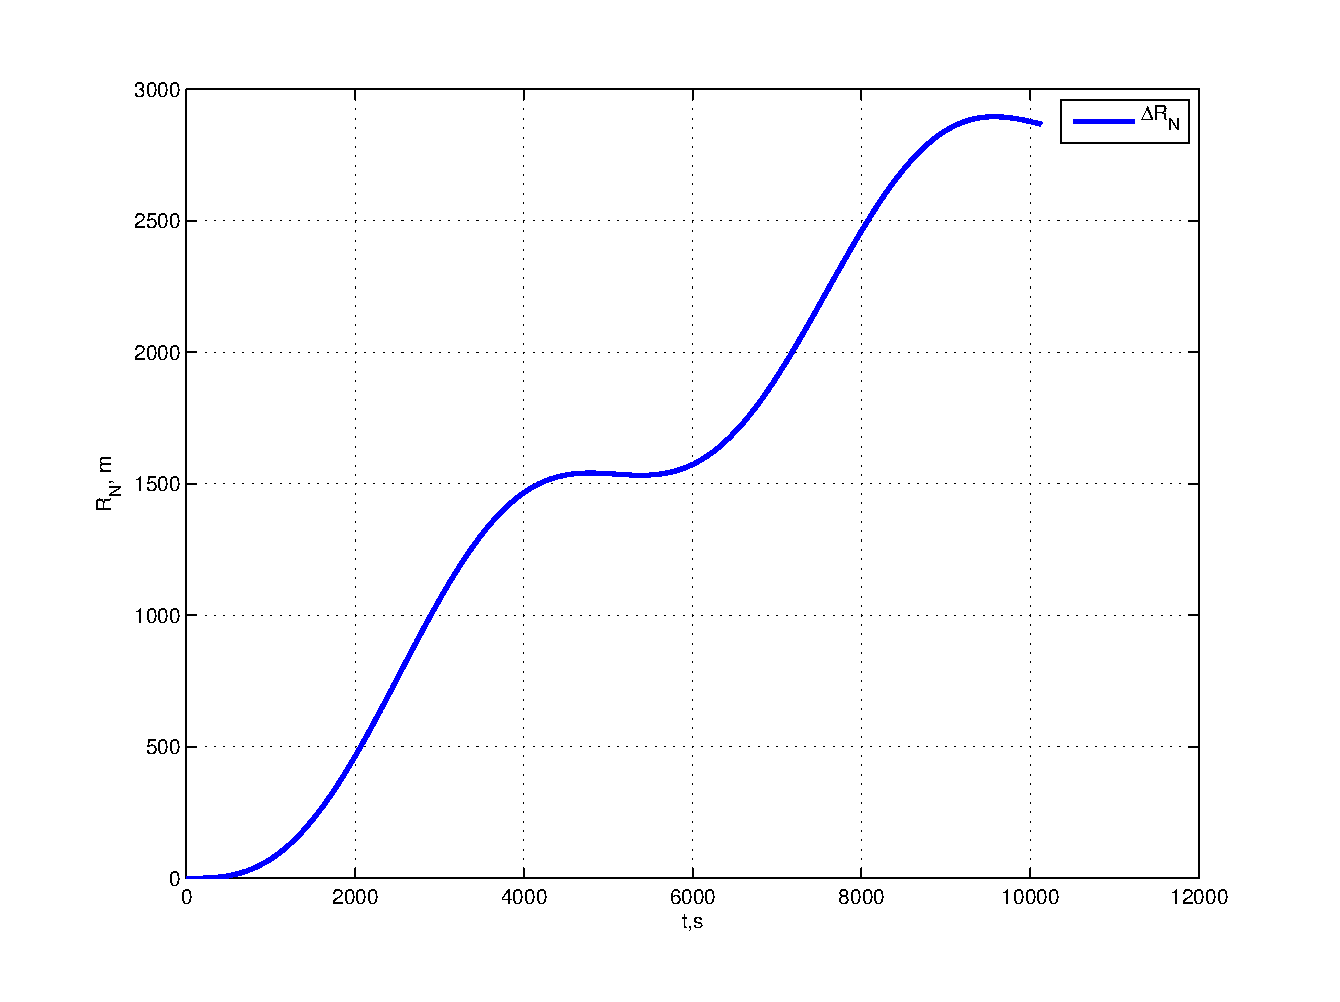
\includegraphics[scale=0.24]{ins_stat_gyro}
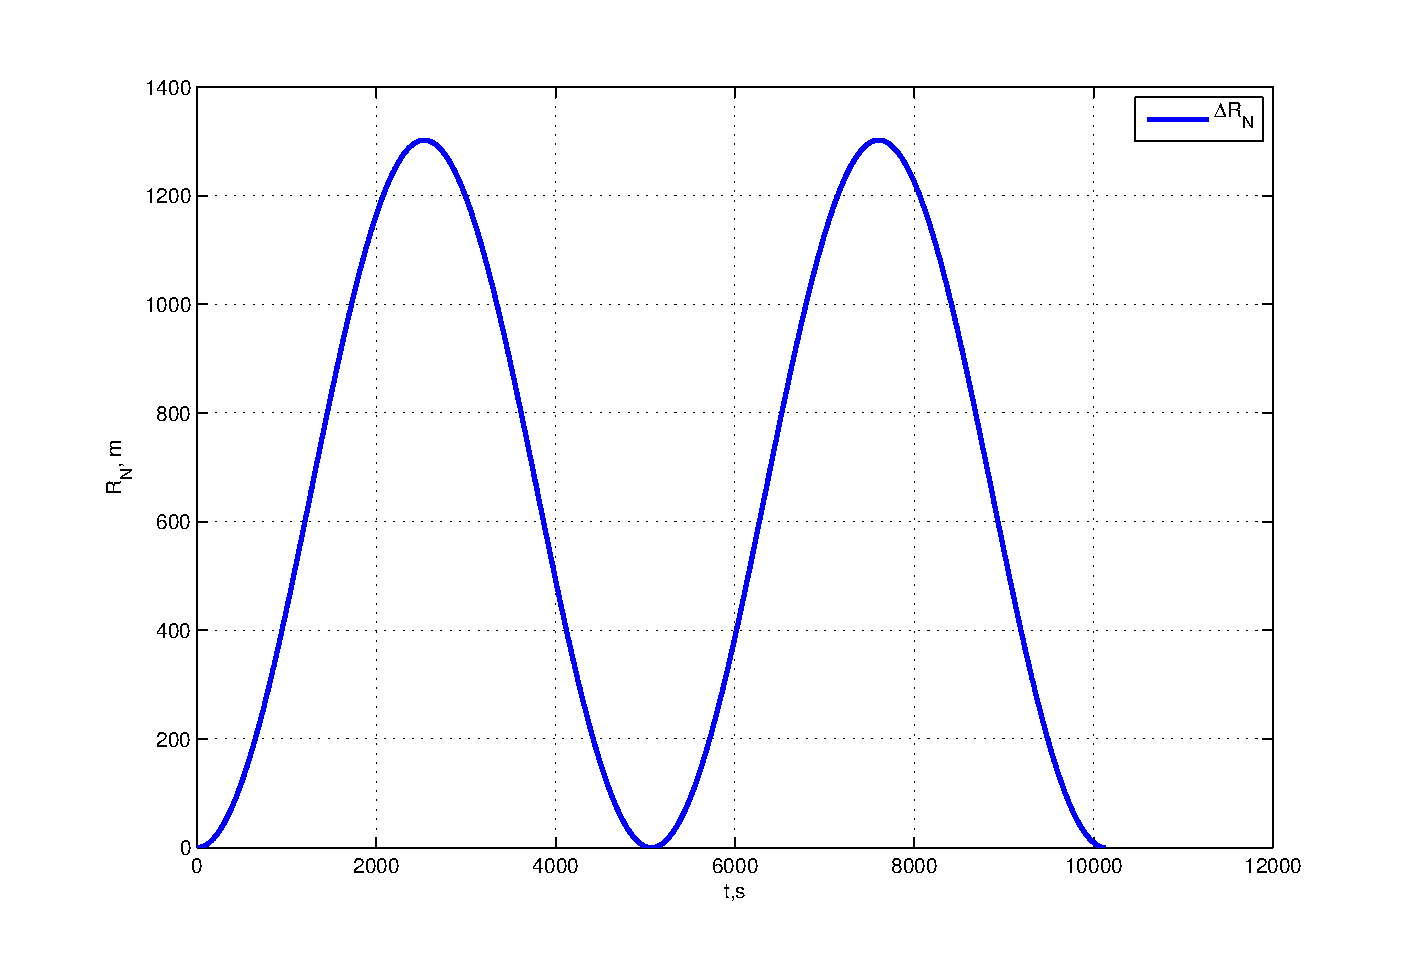
\includegraphics[scale=0.25]{ins_stat_tilt}
\caption{\tiny Еволюція похибки за умови, дрейфу гіроскопа $0.01 deg/h$; Еволюція похибки за умови, похибки координатного тригранника $10^{-3} rad$}
\label{fig:sdins2}
\end{figure}
\end{frame}

%%%%<<<<<<<<<<<<<<<<<<<<<<<<<<<<<<<<<<<<<<<<<<<<<<<<<<<<<<<<<<<<<<<<<<<<<<<<<<<<<<<
\subsection{Сумарна похибка стаціонарно закріпленої БІНС} 
\begin{frame}[plain]
\frametitle{Сумарна похибка стаціонарно закріпленої БІНС}
\begin{figure}[l]
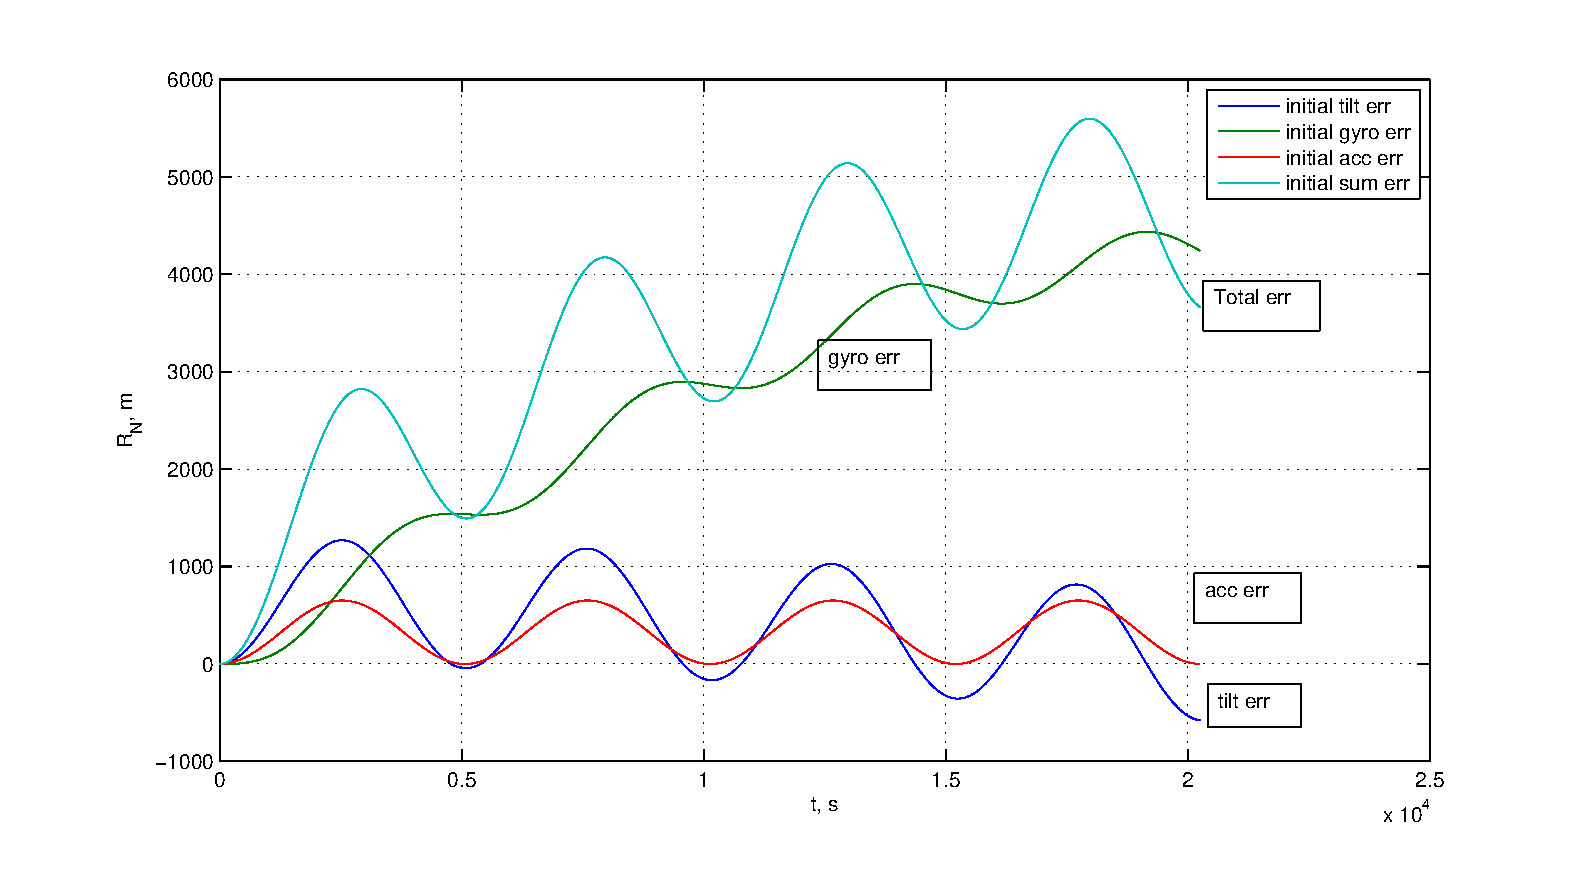
\includegraphics[scale=0.45]{ins_stat_sum}
\caption{\tinyЕволюція сумарної похибки по координаті за умови,
дрейфу гіроскопа   $0.01 deg/h$,похибки координатного тригранника $10^{-3} rad$, та зміщенням акселерометра $10^{-4} m/s^2$}
\label{fig:sdins2}
\end{figure}
\end{frame}
%%%%<<<<<<<<<<<<<<<<<<<<<<<<<<<<<<<<<<<<<<<<<<<<<<<<<<<<<<<<<<<<<<<<<<<<<<<<<<<<<<<
\subsection{Траєкторія руху ЛА тільки за БІНС} 
\begin{frame}%[plain]
\frametitle{Траєкторія руху ЛА тільки за БІНС}
\noindent
\begin{figure}[l]
\noindent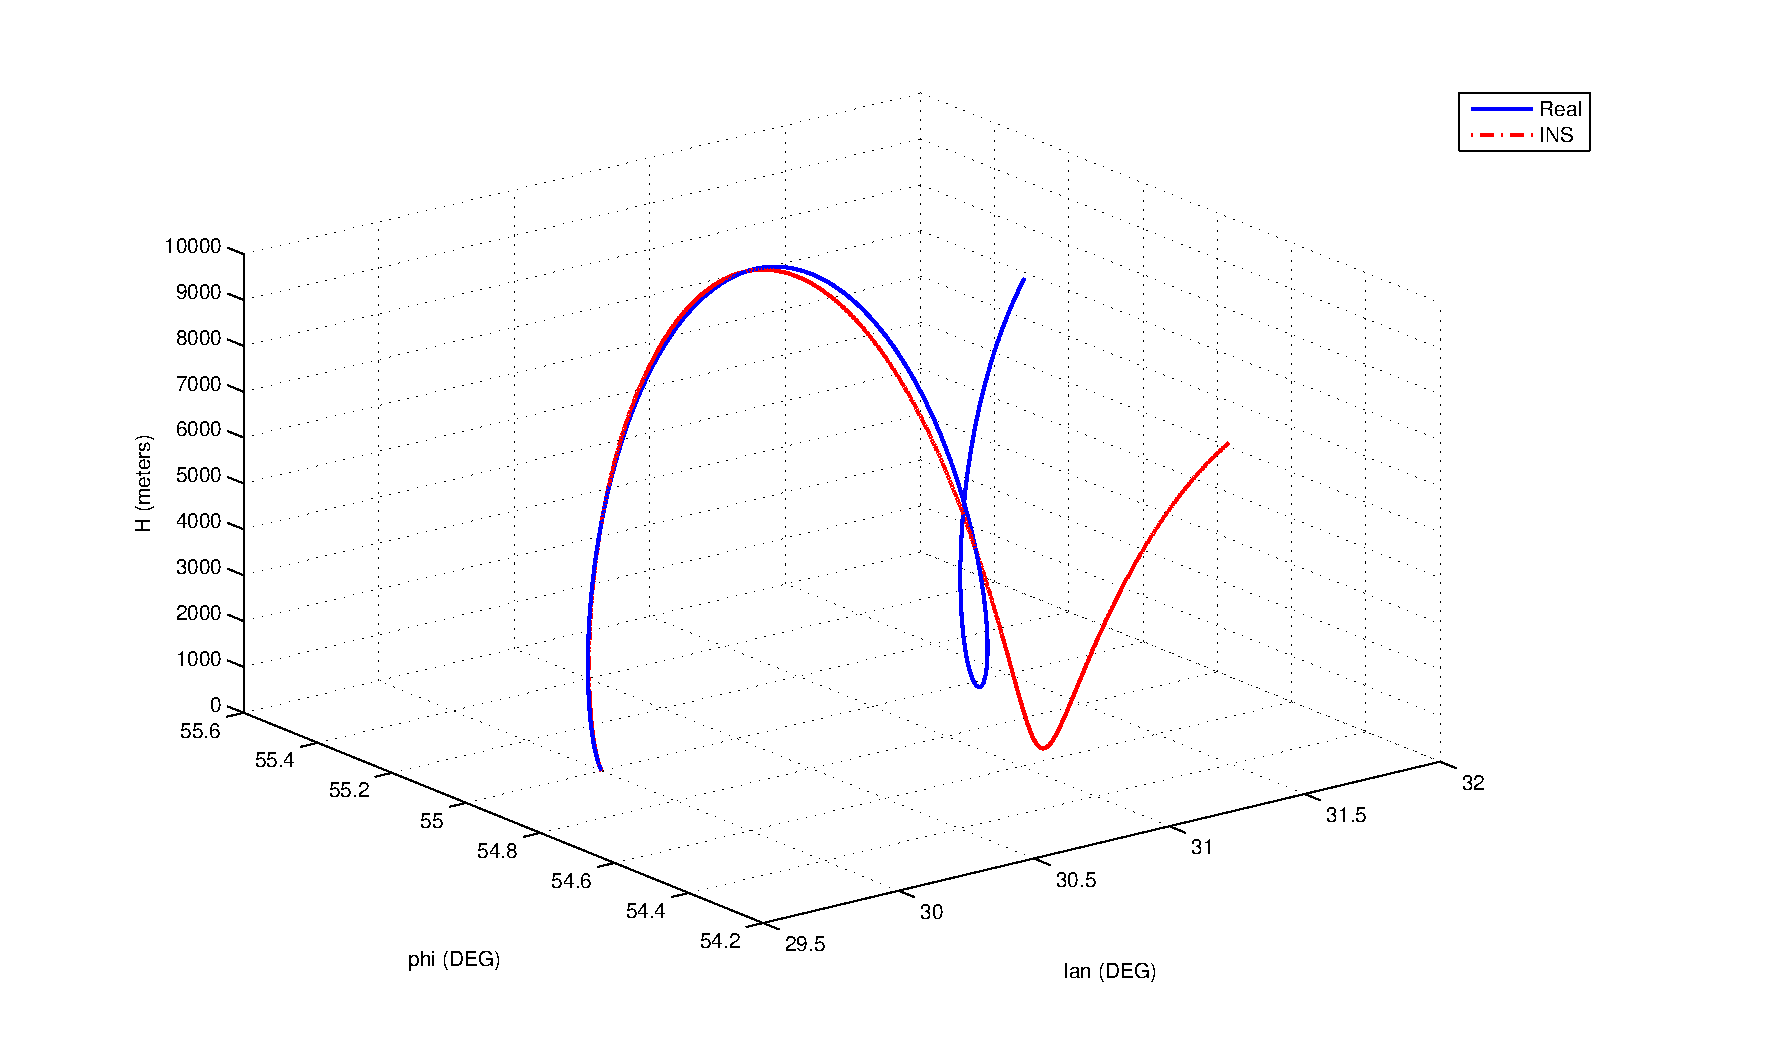
\includegraphics[scale=0.4]{only_ins}
% \caption{\tiny Траєкторія руху ЛА тільки за БІНС }
\end{figure}

\end{frame}
%%%%<<<<<<<<<<<<<<<<<<<<<<<<<<<<<<<<<<<<<<<<<<<<<<<<<<<<<<<<<<<<<<<<<<<<<<<<<<<<<<<
\subsection{Навігаційний фільтр Калмана} 
\begin{frame}[plain]
\frametitle{Навігаційний фільтр Калмана}
\begin{figure}[l]
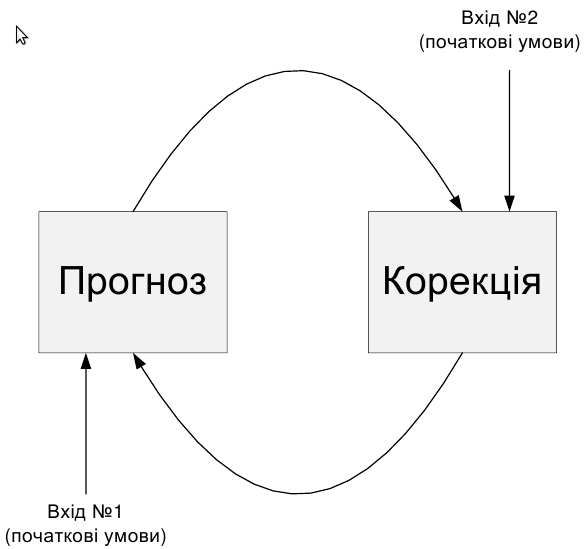
\includegraphics[scale=0.15]{kalman_diag}
% \caption{\tinyЕволюція сумарної }
\end{figure}
\begin{block}{Фільтр Калмана}
\small
Прогноз: \\
$\begin{array}{l} 
{\hat{\bar{X}}_{p,k}(-) =\Phi_{p,k-1} \hat{\bar{X}}_{p,k-1}(+) ,} \\ 
{P_{k}(-) =\Phi_{p,k-1} P_{k-1}(+) \Phi ^{T}_{p,k-1} +G_{p,k-1} G_{p,k-1}^{T} ;} \end{array} $ \\
Корекція:\\
$\begin{array}{l} 
{\hat{\bar{X}}_{p,k}(+)=\hat{\bar{X}}_{p,k}(-) + K_{k} (\bar{Y}_{k} -H\hat{\bar{X}}_{p,k} )} \\ 
{P_{k}(+)={\color{blue}(E-K_{k} H)P_{k}(-) \left(E-K_{k} H\right)^{T}} +{\color{red} K_{k} Q_{p,k} Q_{p,k} ^{T} K_{k}^{T}} } 
\end{array} $ \\
Коефіцієнт Калмана:\\
$K_{k} =P_{k}(-) H^{T} (HP_{k}(-) H^{T} +Q_{p,k} Q_{p,k} ^{T} )^{-1} $
\end{block}
\end{frame}

%%%%<<<<<<<<<<<<<<<<<<<<<<<<<<<<<<<<<<<<<<<<<<<<<<<<<<<<<<<<<<<<<<<<<<<<<<<<<<<<<<<
\subsection{Траєкторія руху ЛА} 
\begin{frame}%[plain]
\frametitle{Траєкторія руху ЛА та кути крену, курса і тангажа}
\noindent
\begin{figure}[l]
\noindent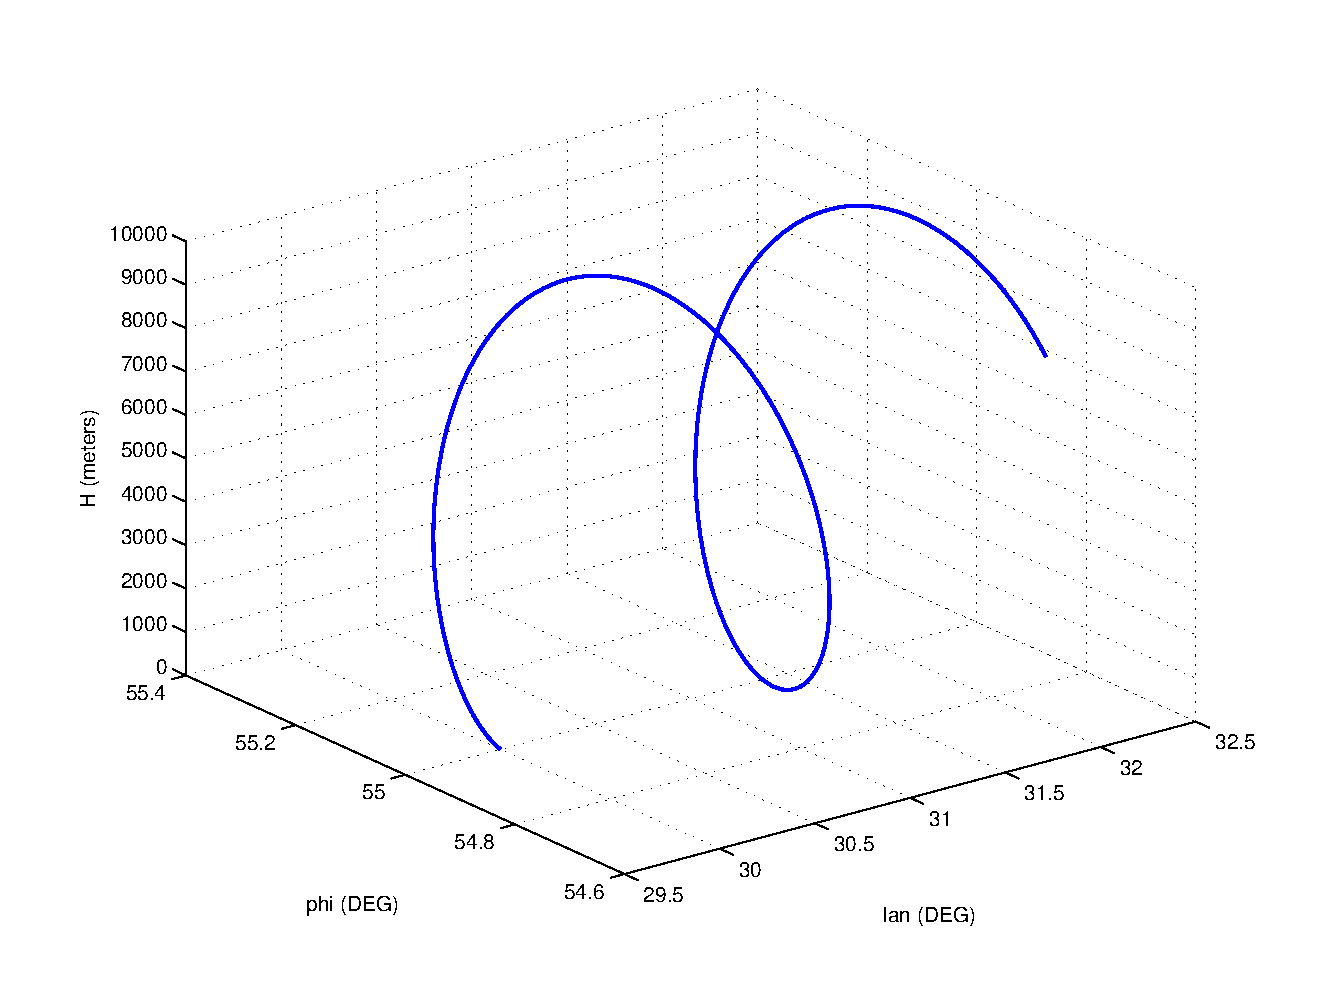
\includegraphics[scale=0.28]{path_3d}
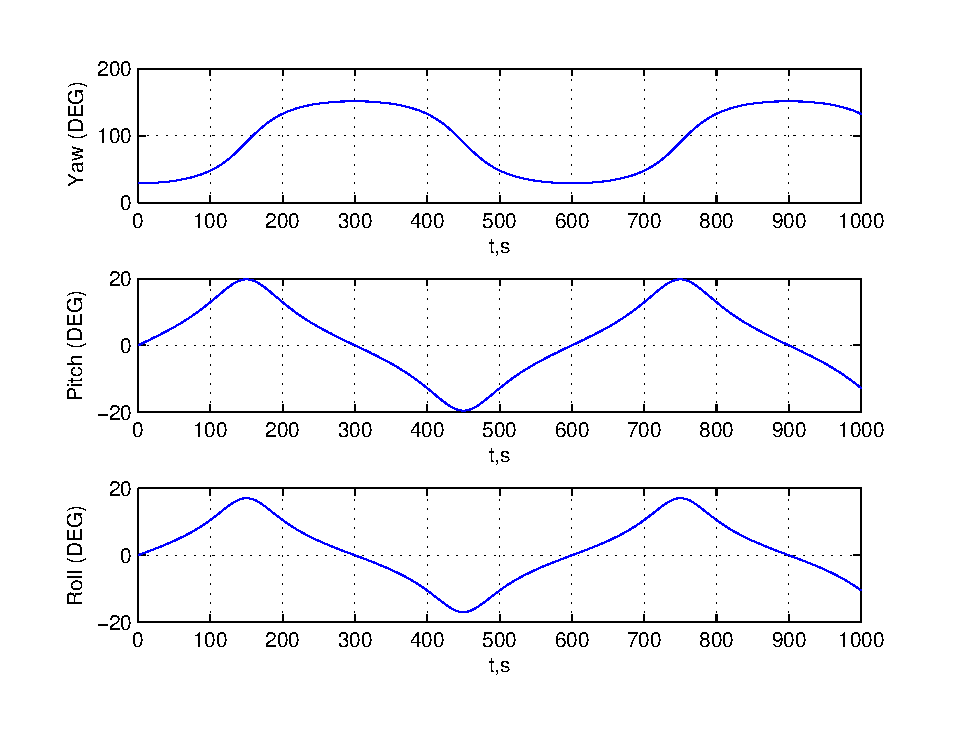
\includegraphics[scale=0.35]{path_PYR}
\caption{\tiny Траєкторія руху ЛА та його кути орієнтації }
\end{figure}

\end{frame}

%%%%<<<<<<<<<<<<<<<<<<<<<<<<<<<<<<<<<<<<<<<<<<<<<<<<<<<<<<<<<<<<<<<<<<<<<<<<<<<<<<<
\section{Результати моделювання ІСНС} 
\subsection{Поихибка оцінки по координаті} 
\begin{frame}%[plain]
\frametitle{Поихибка оцінки по координаті}
\noindent
\begin{figure}
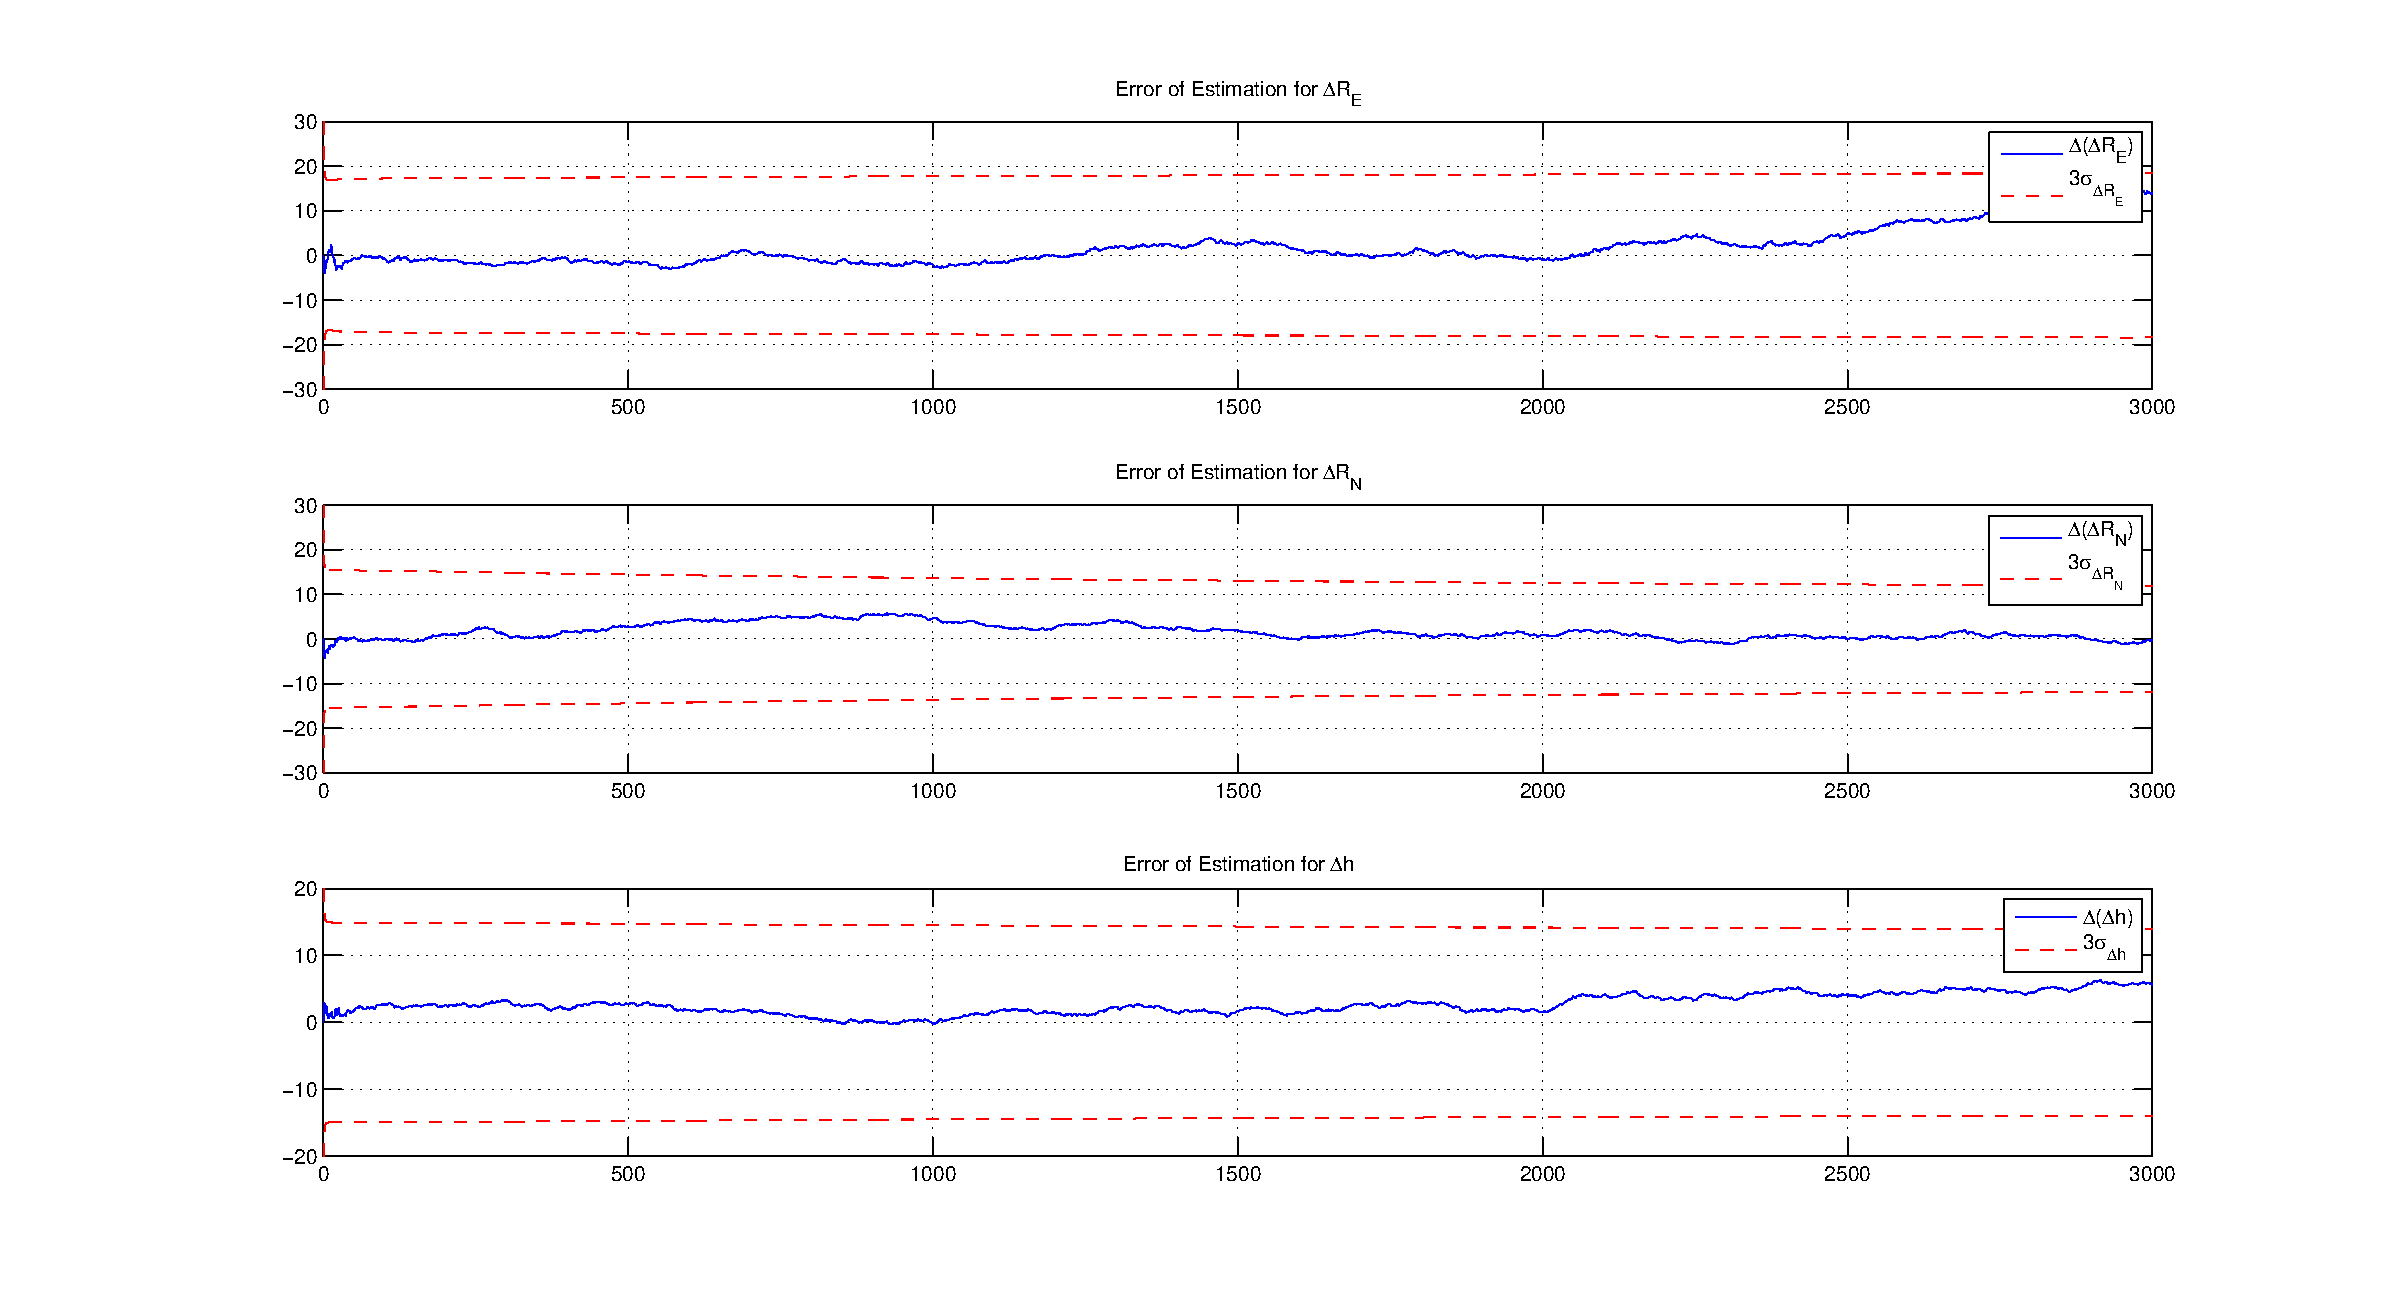
\includegraphics[scale=0.3]{ErrEstCovR}
% \caption{\tiny Траєкторія руху ЛА та його кути орієнтації }
\end{figure}
\end{frame}

%%%%<<<<<<<<<<<<<<<<<<<<<<<<<<<<<<<<<<<<<<<<<<<<<<<<<<<<<<<<<<<<<<<<<<<<<<<<<<<<<<<
\subsection{Поихибка оцінки по швидкості} 
\begin{frame}%[plain]
\frametitle{Поихибка оцінки по швидкості}
\noindent
\begin{figure}
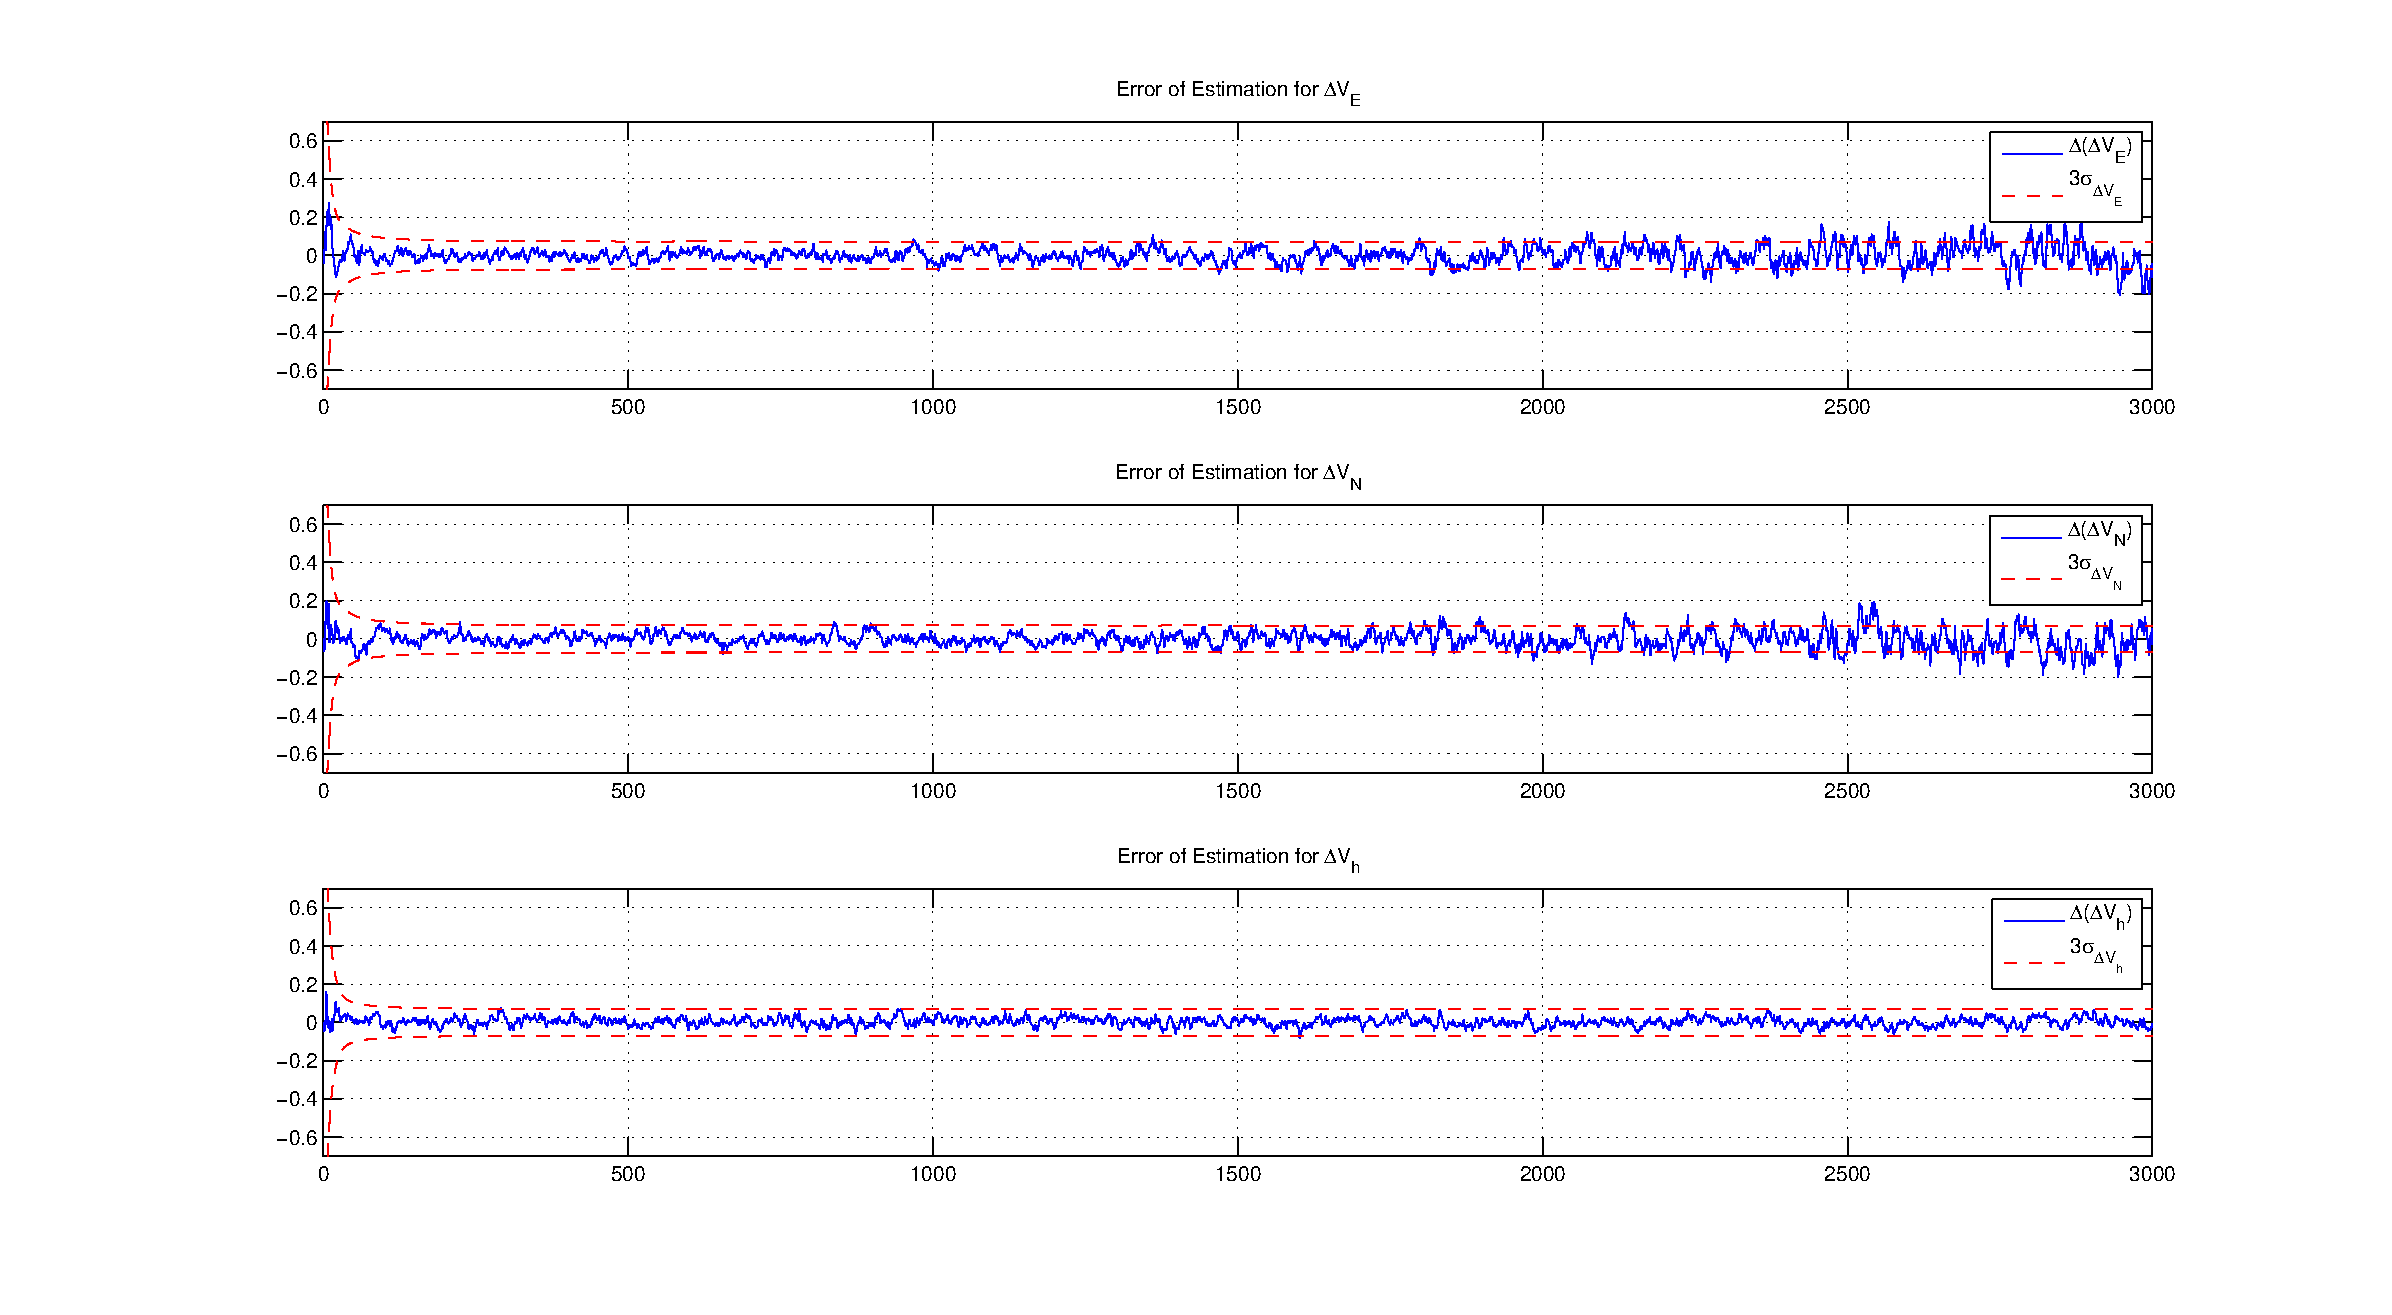
\includegraphics[scale=0.3]{ErrEstCovV}
% \caption{\tiny Траєкторія руху ЛА та його кути орієнтації }
\end{figure}
\end{frame}

%%%%<<<<<<<<<<<<<<<<<<<<<<<<<<<<<<<<<<<<<<<<<<<<<<<<<<<<<<<<<<<<<<<<<<<<<<<<<<<<<<<
\subsection{Поихибка оцінки по орієнтації} 
\begin{frame}%[plain]
\frametitle{Поихибка оцінки по орієнтації}
\noindent
\begin{figure}
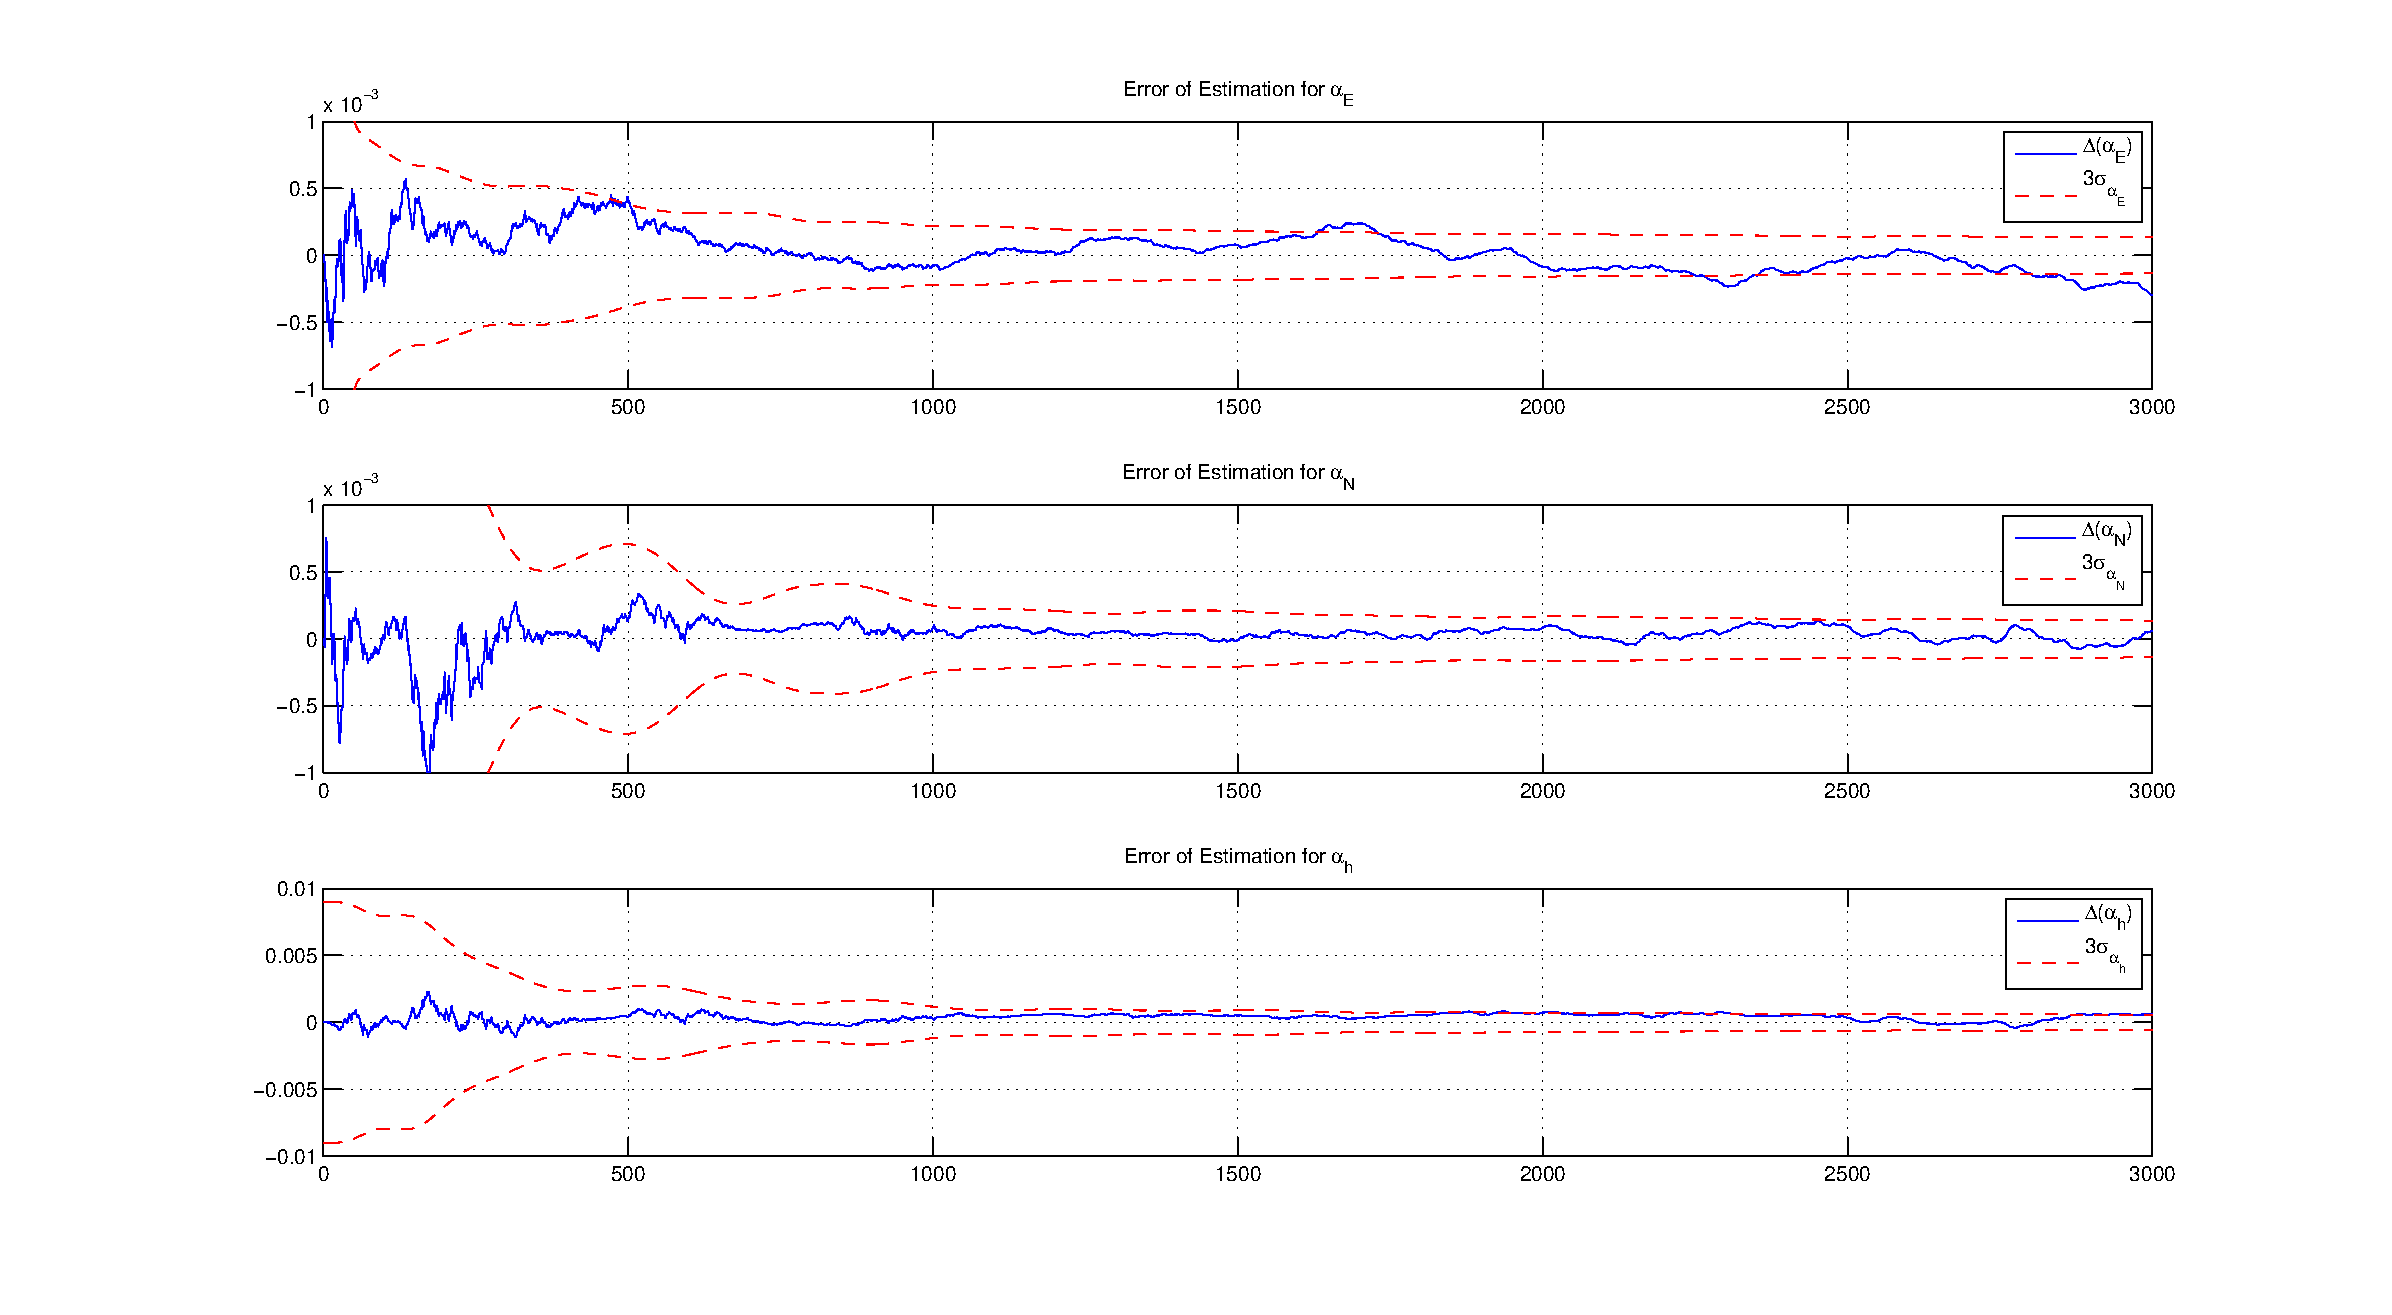
\includegraphics[scale=0.3]{ErrEstCovAlph}
% \caption{\tiny Траєкторія руху ЛА та його кути орієнтації }
\end{figure}
\end{frame}

%%%%<<<<<<<<<<<<<<<<<<<<<<<<<<<<<<<<<<<<<<<<<<<<<<<<<<<<<<<<<<<<<<<<<<<<<<<<<<<<<<<
\subsection{Поихибка оцінки дрейфів гіроскопів} 
\begin{frame}%[plain]
\frametitle{Поихибка оцінки дрейфів гіроскопів}
\noindent
\begin{figure}
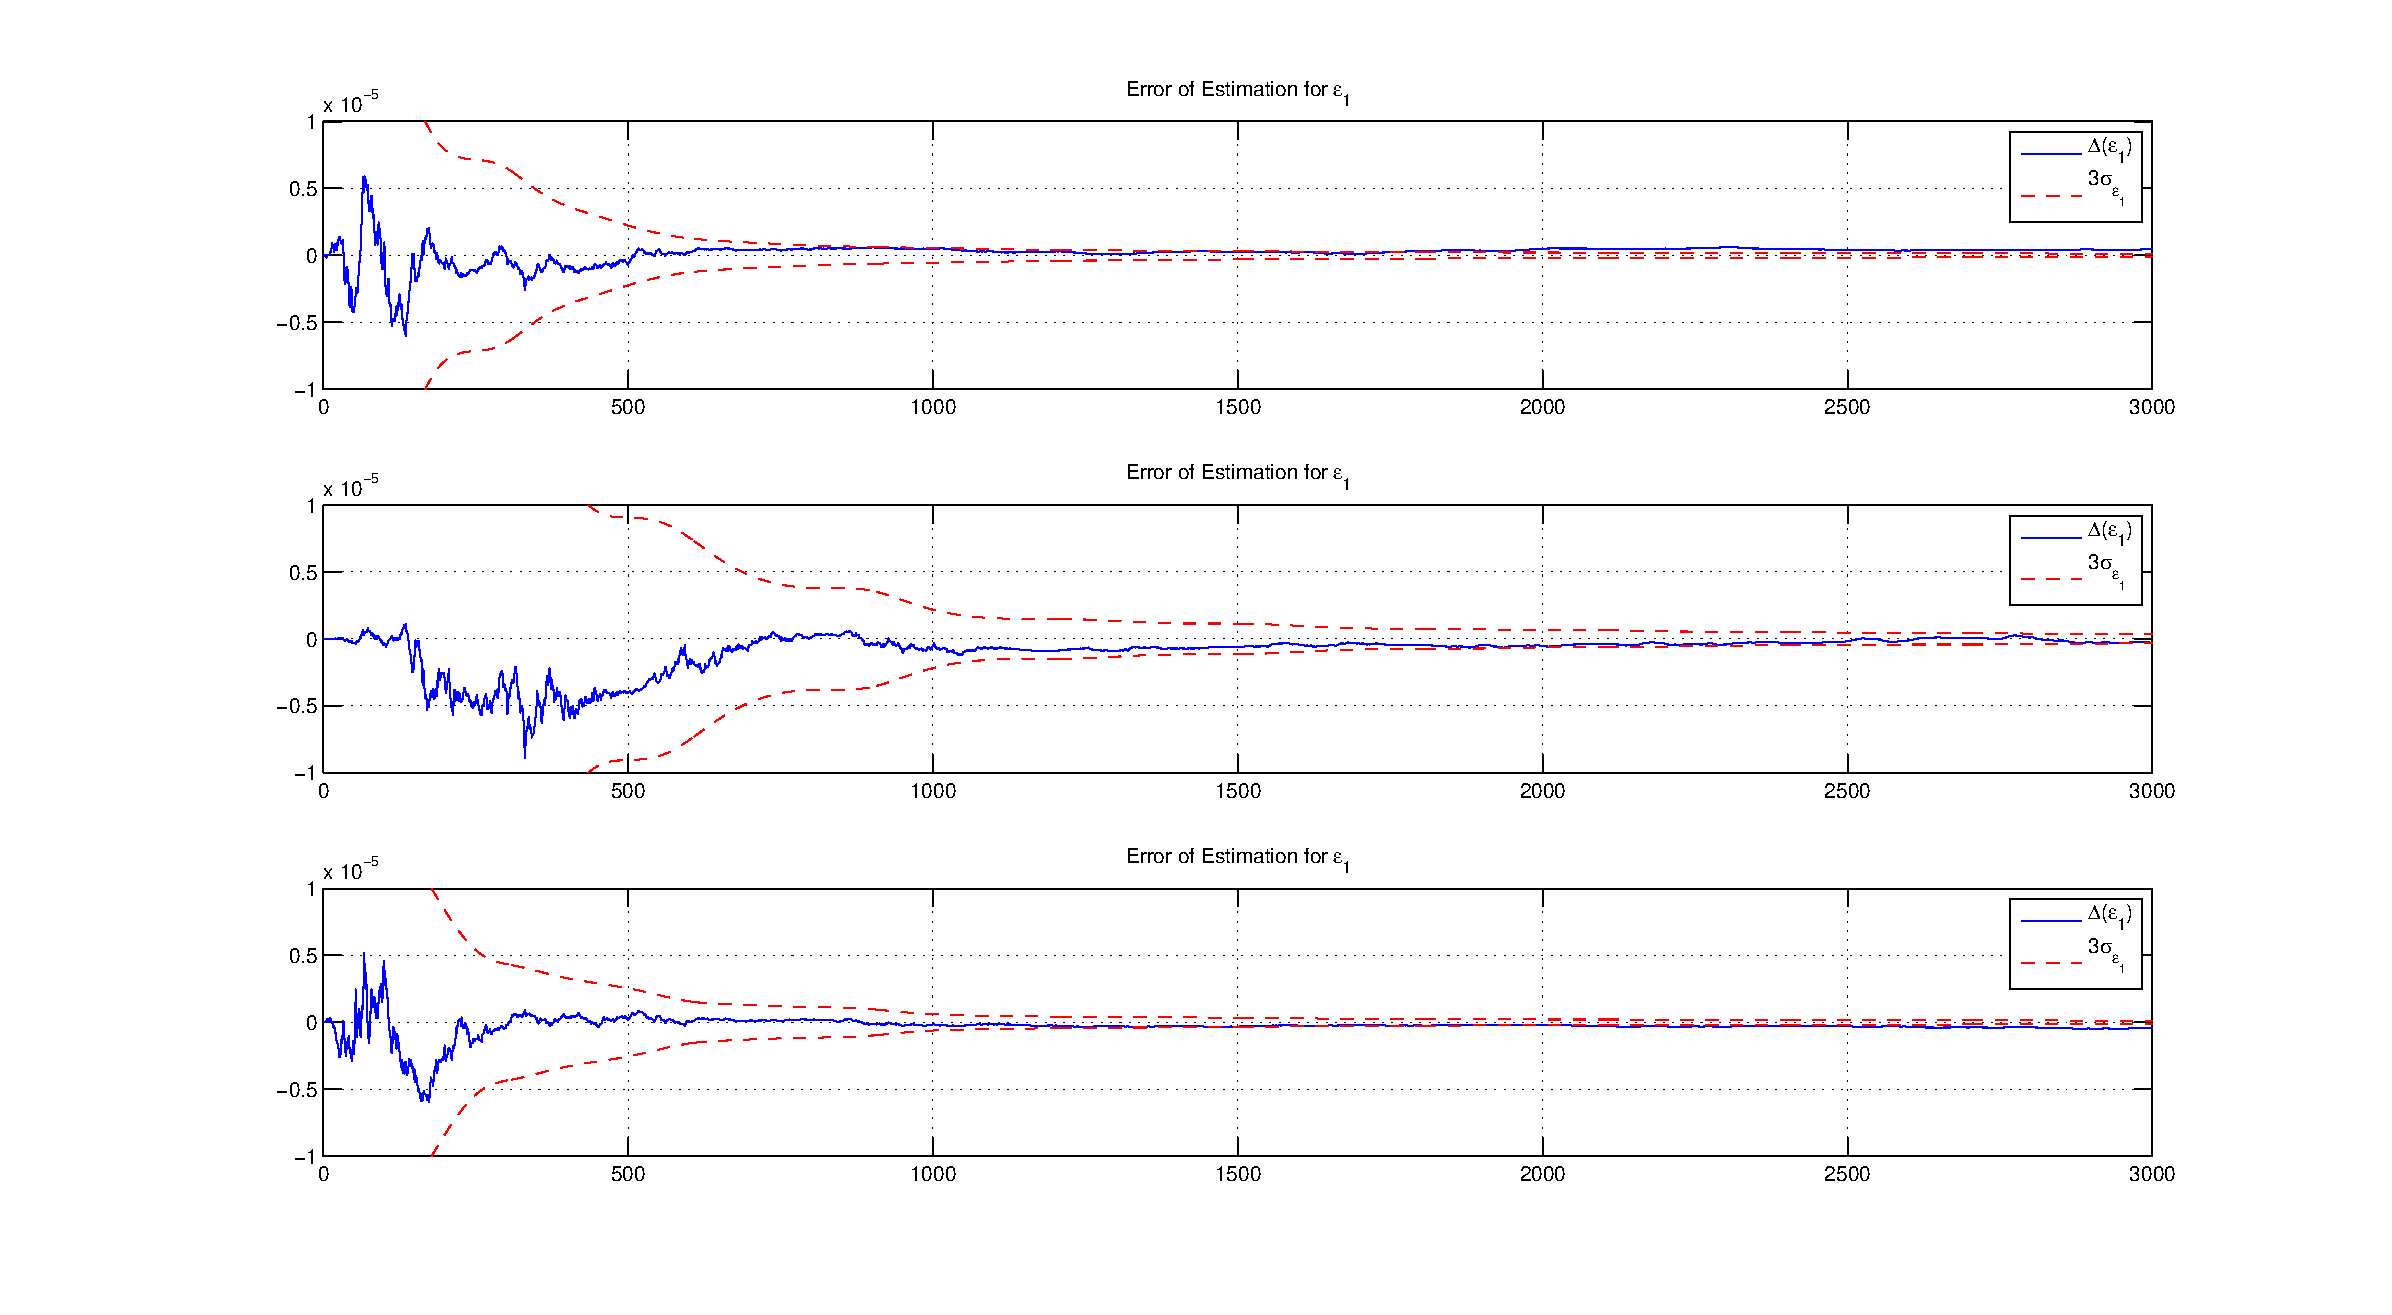
\includegraphics[scale=0.3]{ErrEstCovGyro}
% \caption{\tiny Траєкторія руху ЛА та його кути орієнтації }
\end{figure}
\end{frame}

%%%%<<<<<<<<<<<<<<<<<<<<<<<<<<<<<<<<<<<<<<<<<<<<<<<<<<<<<<<<<<<<<<<<<<<<<<<<<<<<<<<
\subsection{Поихибка оцінки зміщення акселерометрів} 
\begin{frame}%[plain]
\frametitle{Поихибка оцінки зміщення акселерометрів}
\begin{figure}
\centering
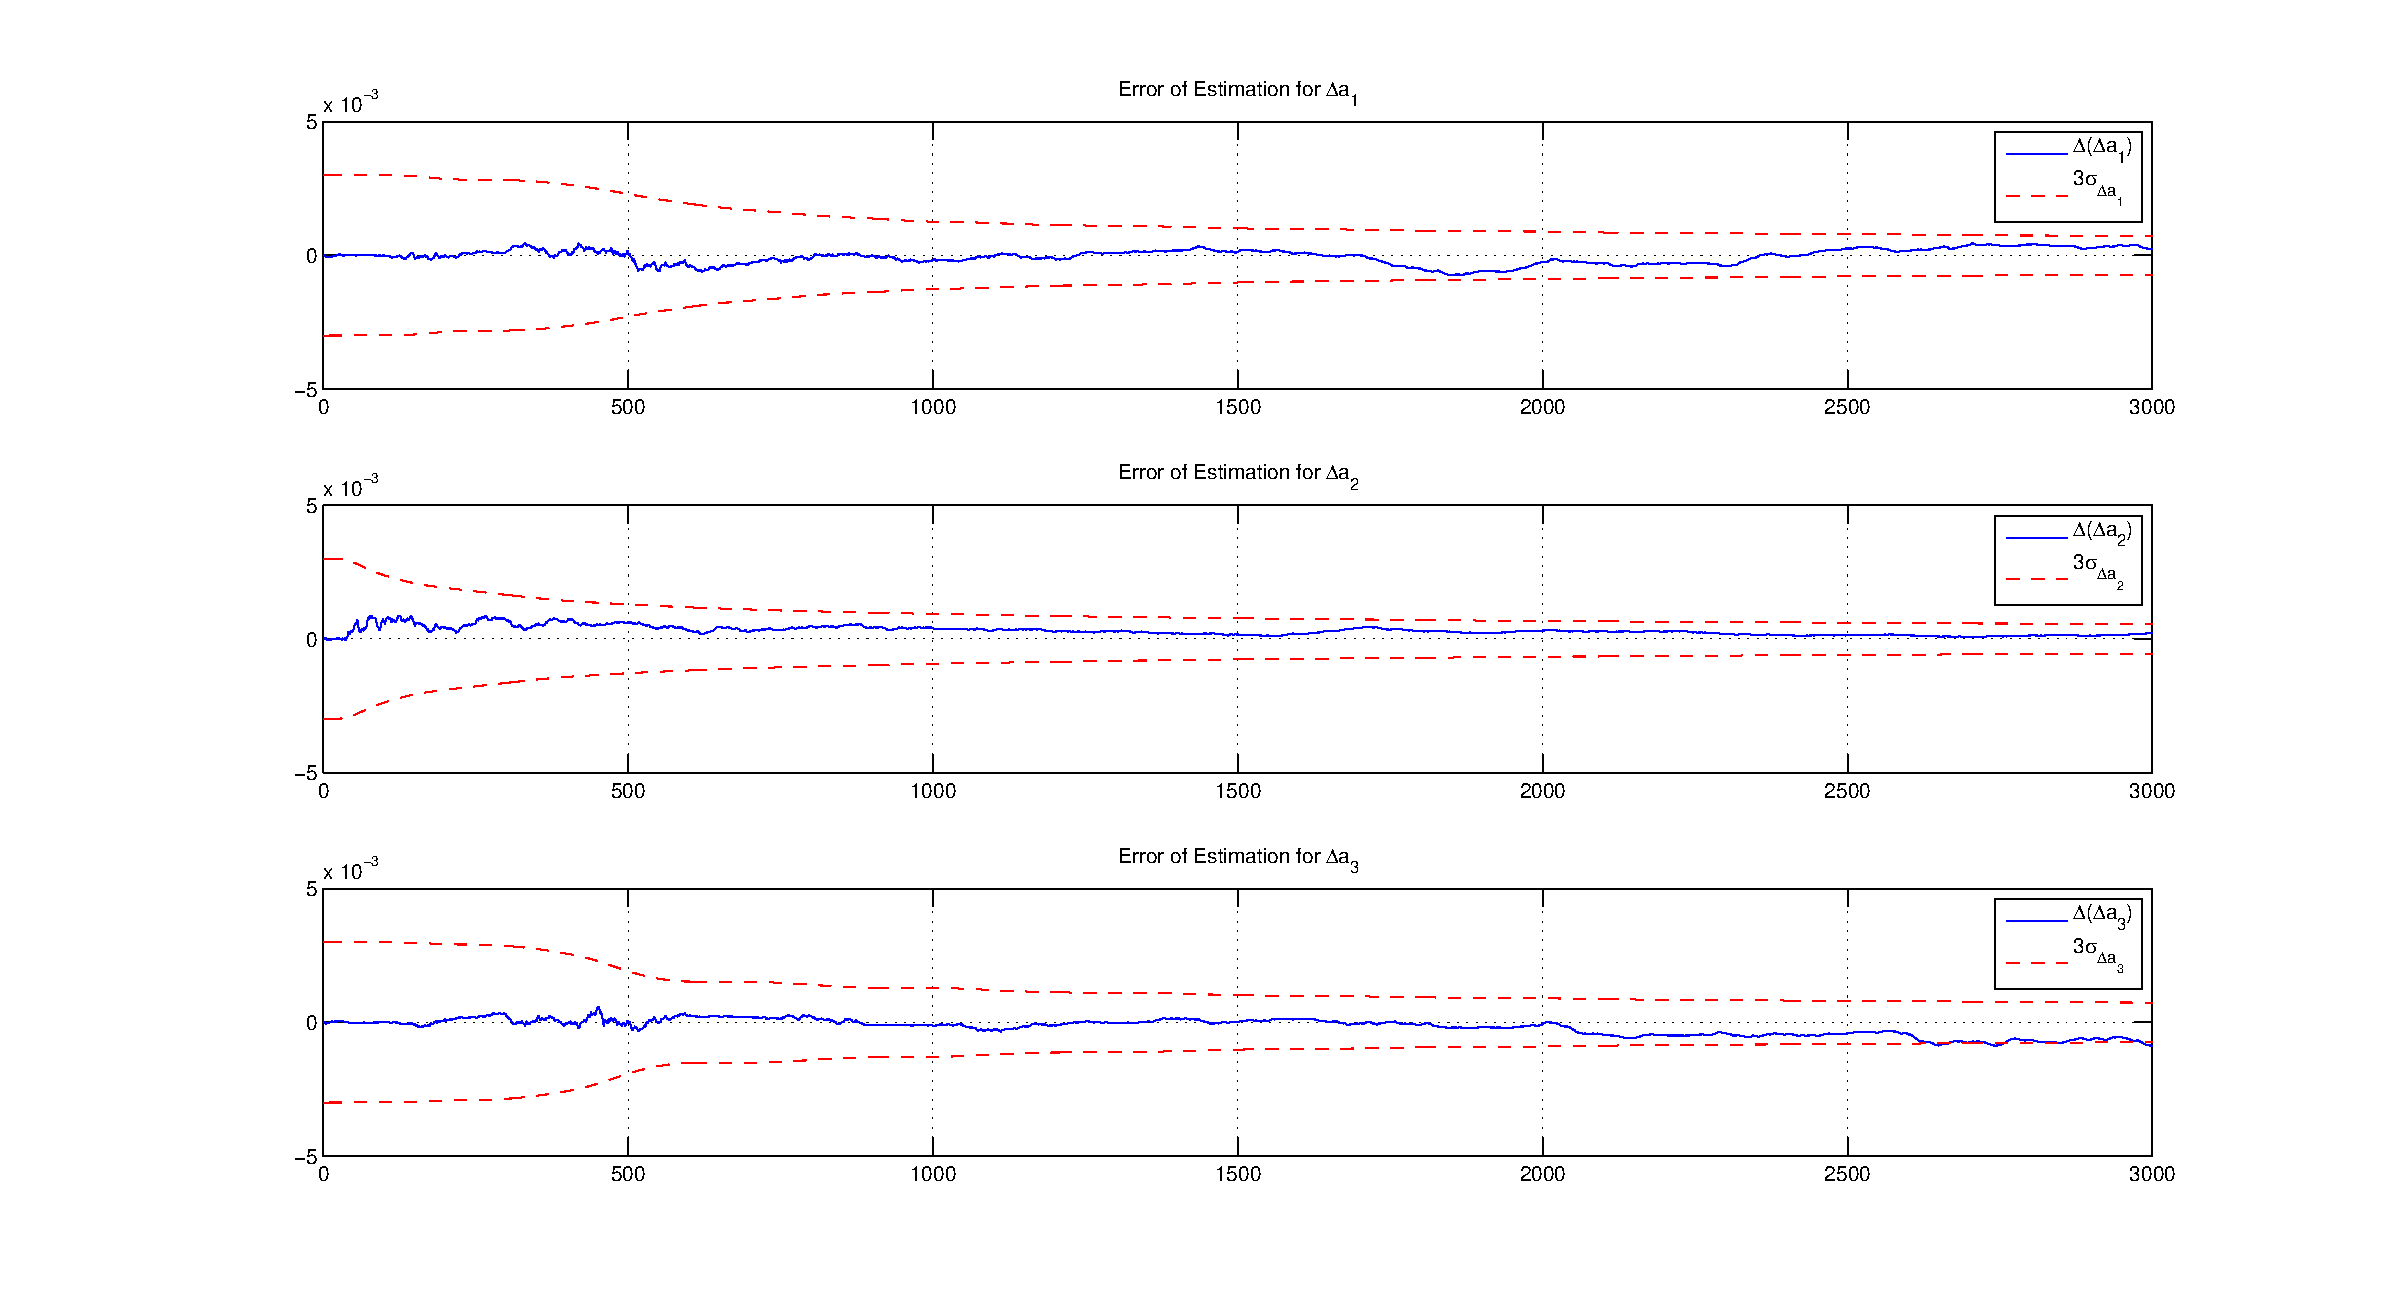
\includegraphics[scale=0.3]{ErrEstCovAcc}
% \caption{\tiny Траєкторія руху ЛА та його кути орієнтації }
\end{figure}
\end{frame}
%%%%<<<<<<<<<<<<<<<<<<<<<<<<<<<<<<<<<<<<<<<<<<<<<<<<<<<<<<<<<<<<<<<<<<<<<<<<<<<<<<<
\subsection{Поихибка оцінки курсу, крена, тангажа} 
\begin{frame}%[plain]
\frametitle{Поихибка оцінки курсу, крена, тангажа}
\begin{figure}
\centering
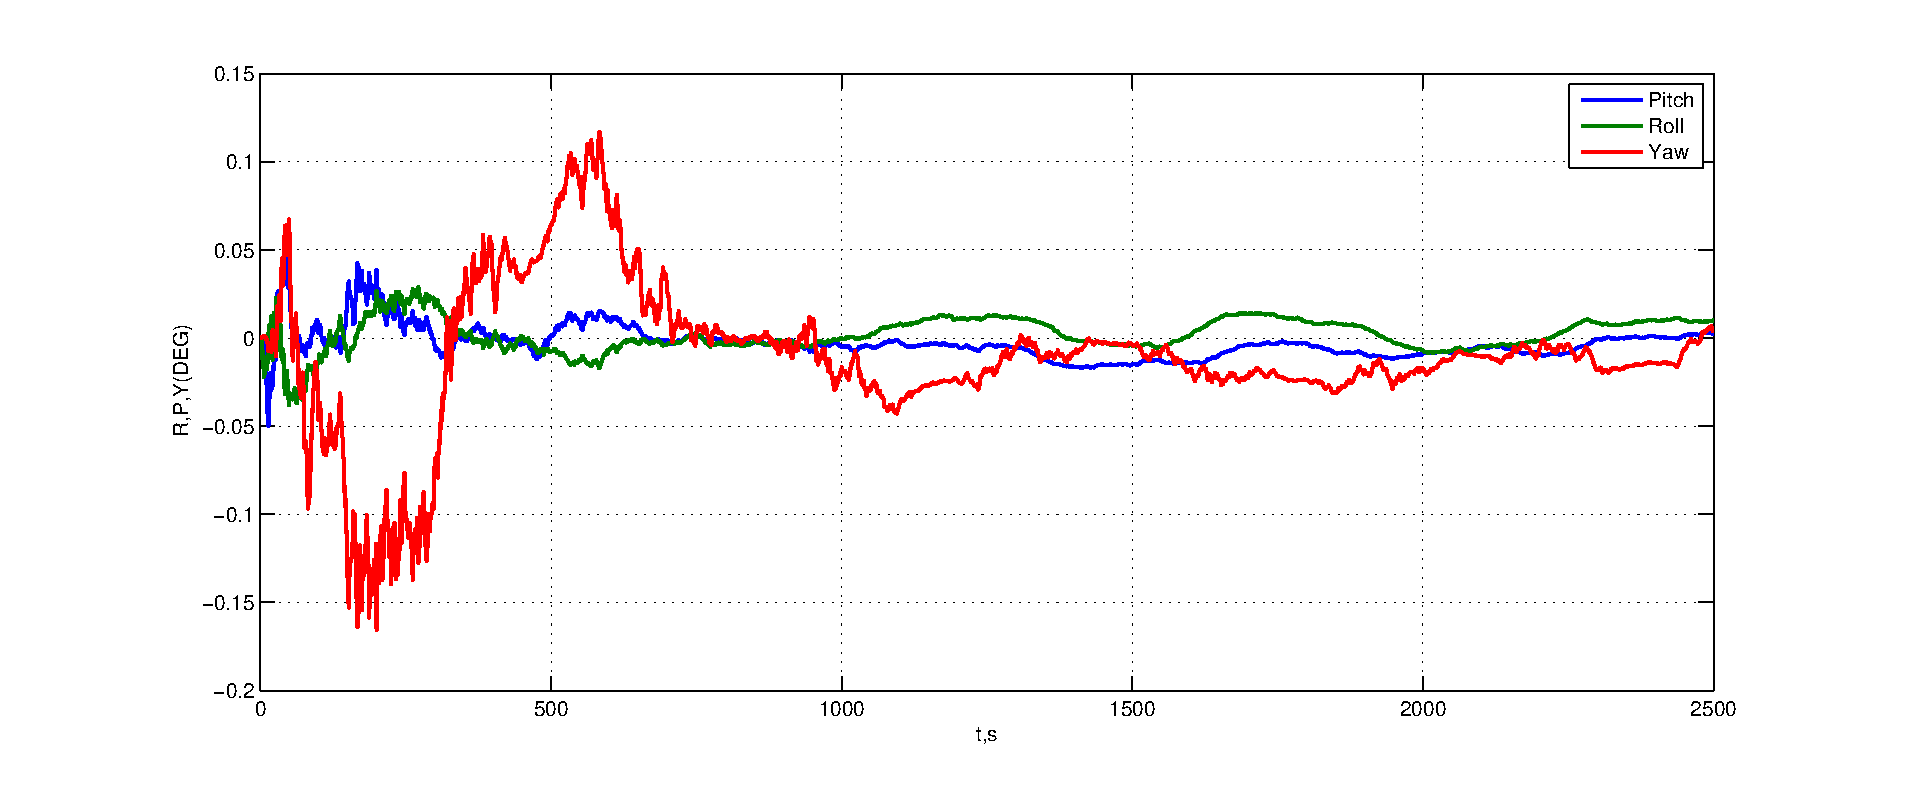
\includegraphics[scale=0.4]{ErrEstAngle2}
% \caption{\tiny Траєкторія руху ЛА та його кути орієнтації }
\end{figure}
\end{frame}
%%%%<<<<<<<<<<<<<<<<<<<<<<<<<<<<<<<<<<<<<<<<<<<<<<<<<<<<<<<<<<<<<<<<<<<<<<<<<<<<<<<
\subsection{Сходимість коваріацій параметрів} 
\begin{frame}%[plain]
\frametitle{Сходимість коваріацій параметрів}
\begin{figure}
\centering
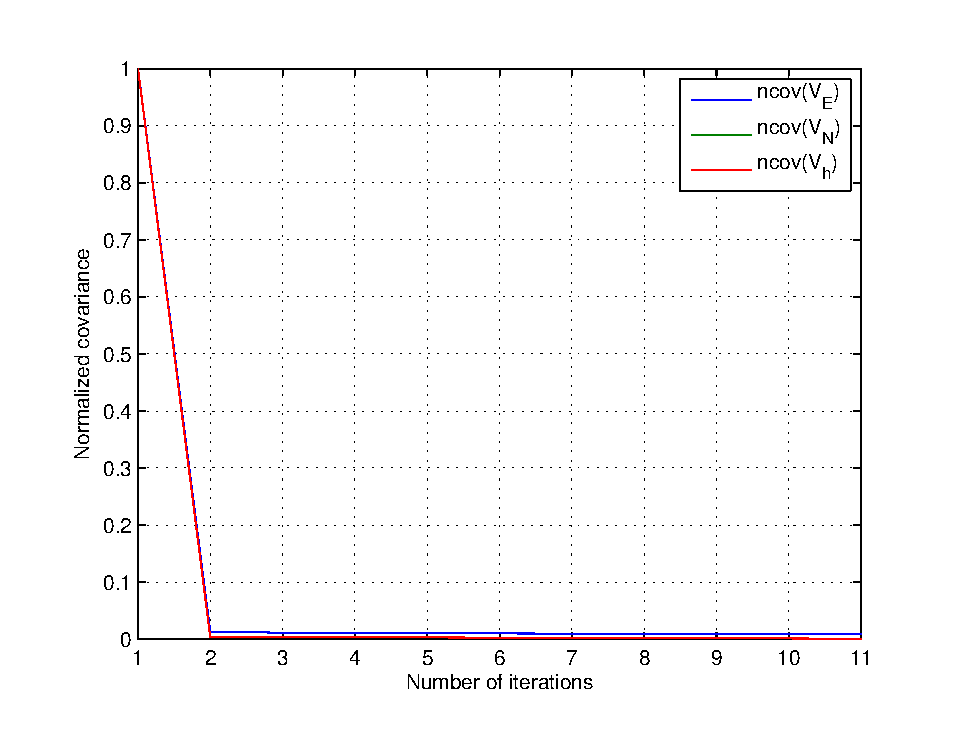
\includegraphics[ width=60mm, height=30.0mm]{cov_v}
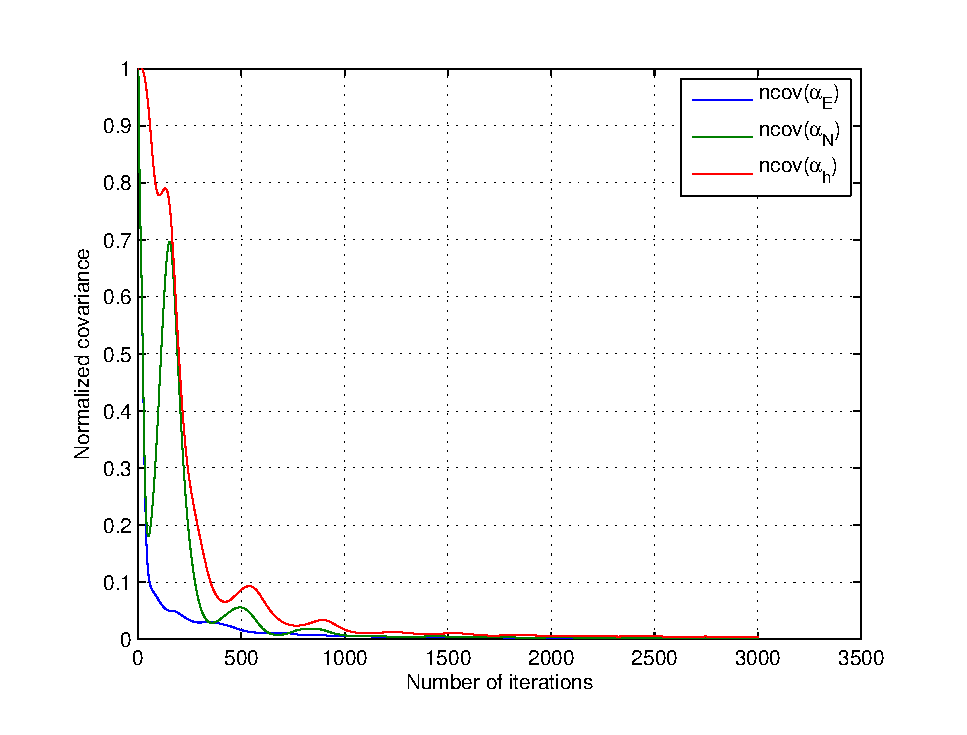
\includegraphics[ width=60mm, height=30.0mm]{cov_alpha}\\
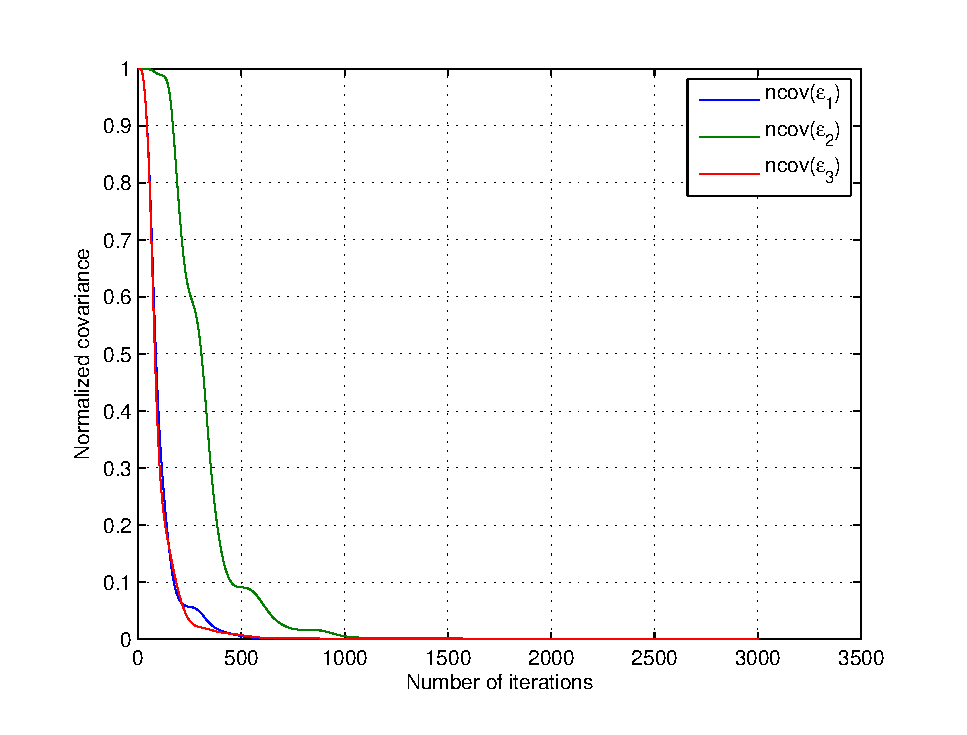
\includegraphics[ width=60mm, height=30.0mm]{cov_eps}
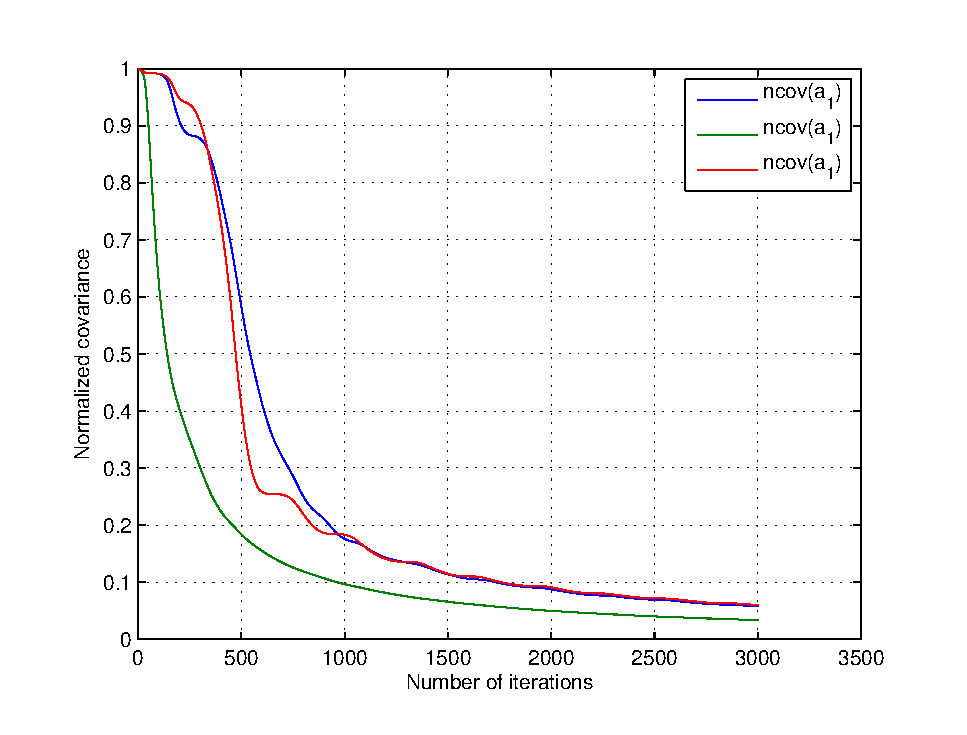
\includegraphics[ width=60mm, height=30.0mm]{cov_a}
\caption{\tiny Сходимість нормалізованих коваріацій швидкостей, орієнтації, дрейфу гіроскопів та зміщення акселерометрів}
\end{figure}
\end{frame}
%%%%<<<<<<<<<<<<<<<<<<<<<<<<<<<<<<<<<<<<<<<<<<<<<<<<<<<<<<<<<<<<<<<<<<<<<<<<<<<<<<<
\subsection{Траєкторія руху ЛА за БІНС і ФК} 
\begin{frame}%[plain]
\frametitle{Траєкторія руху за БІНС і ФК}
\noindent
\begin{figure}[l]
% \noindent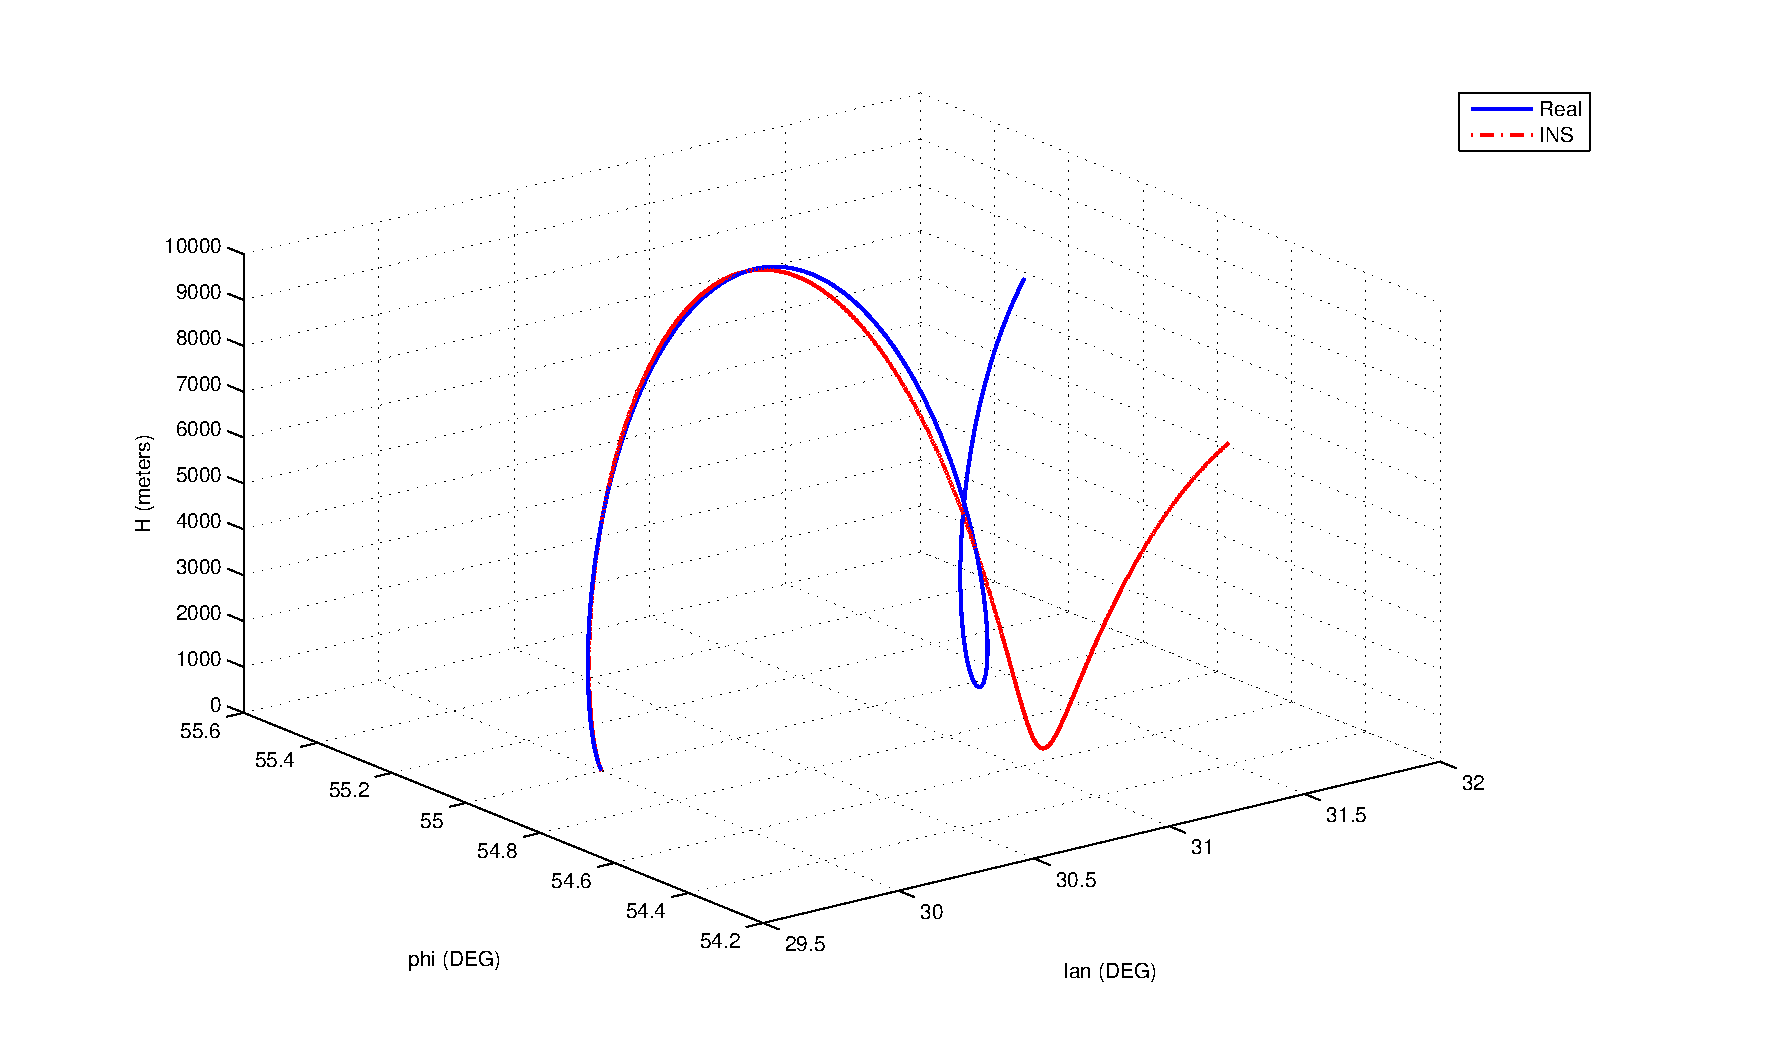
\includegraphics[scale=0.2]{only_ins}
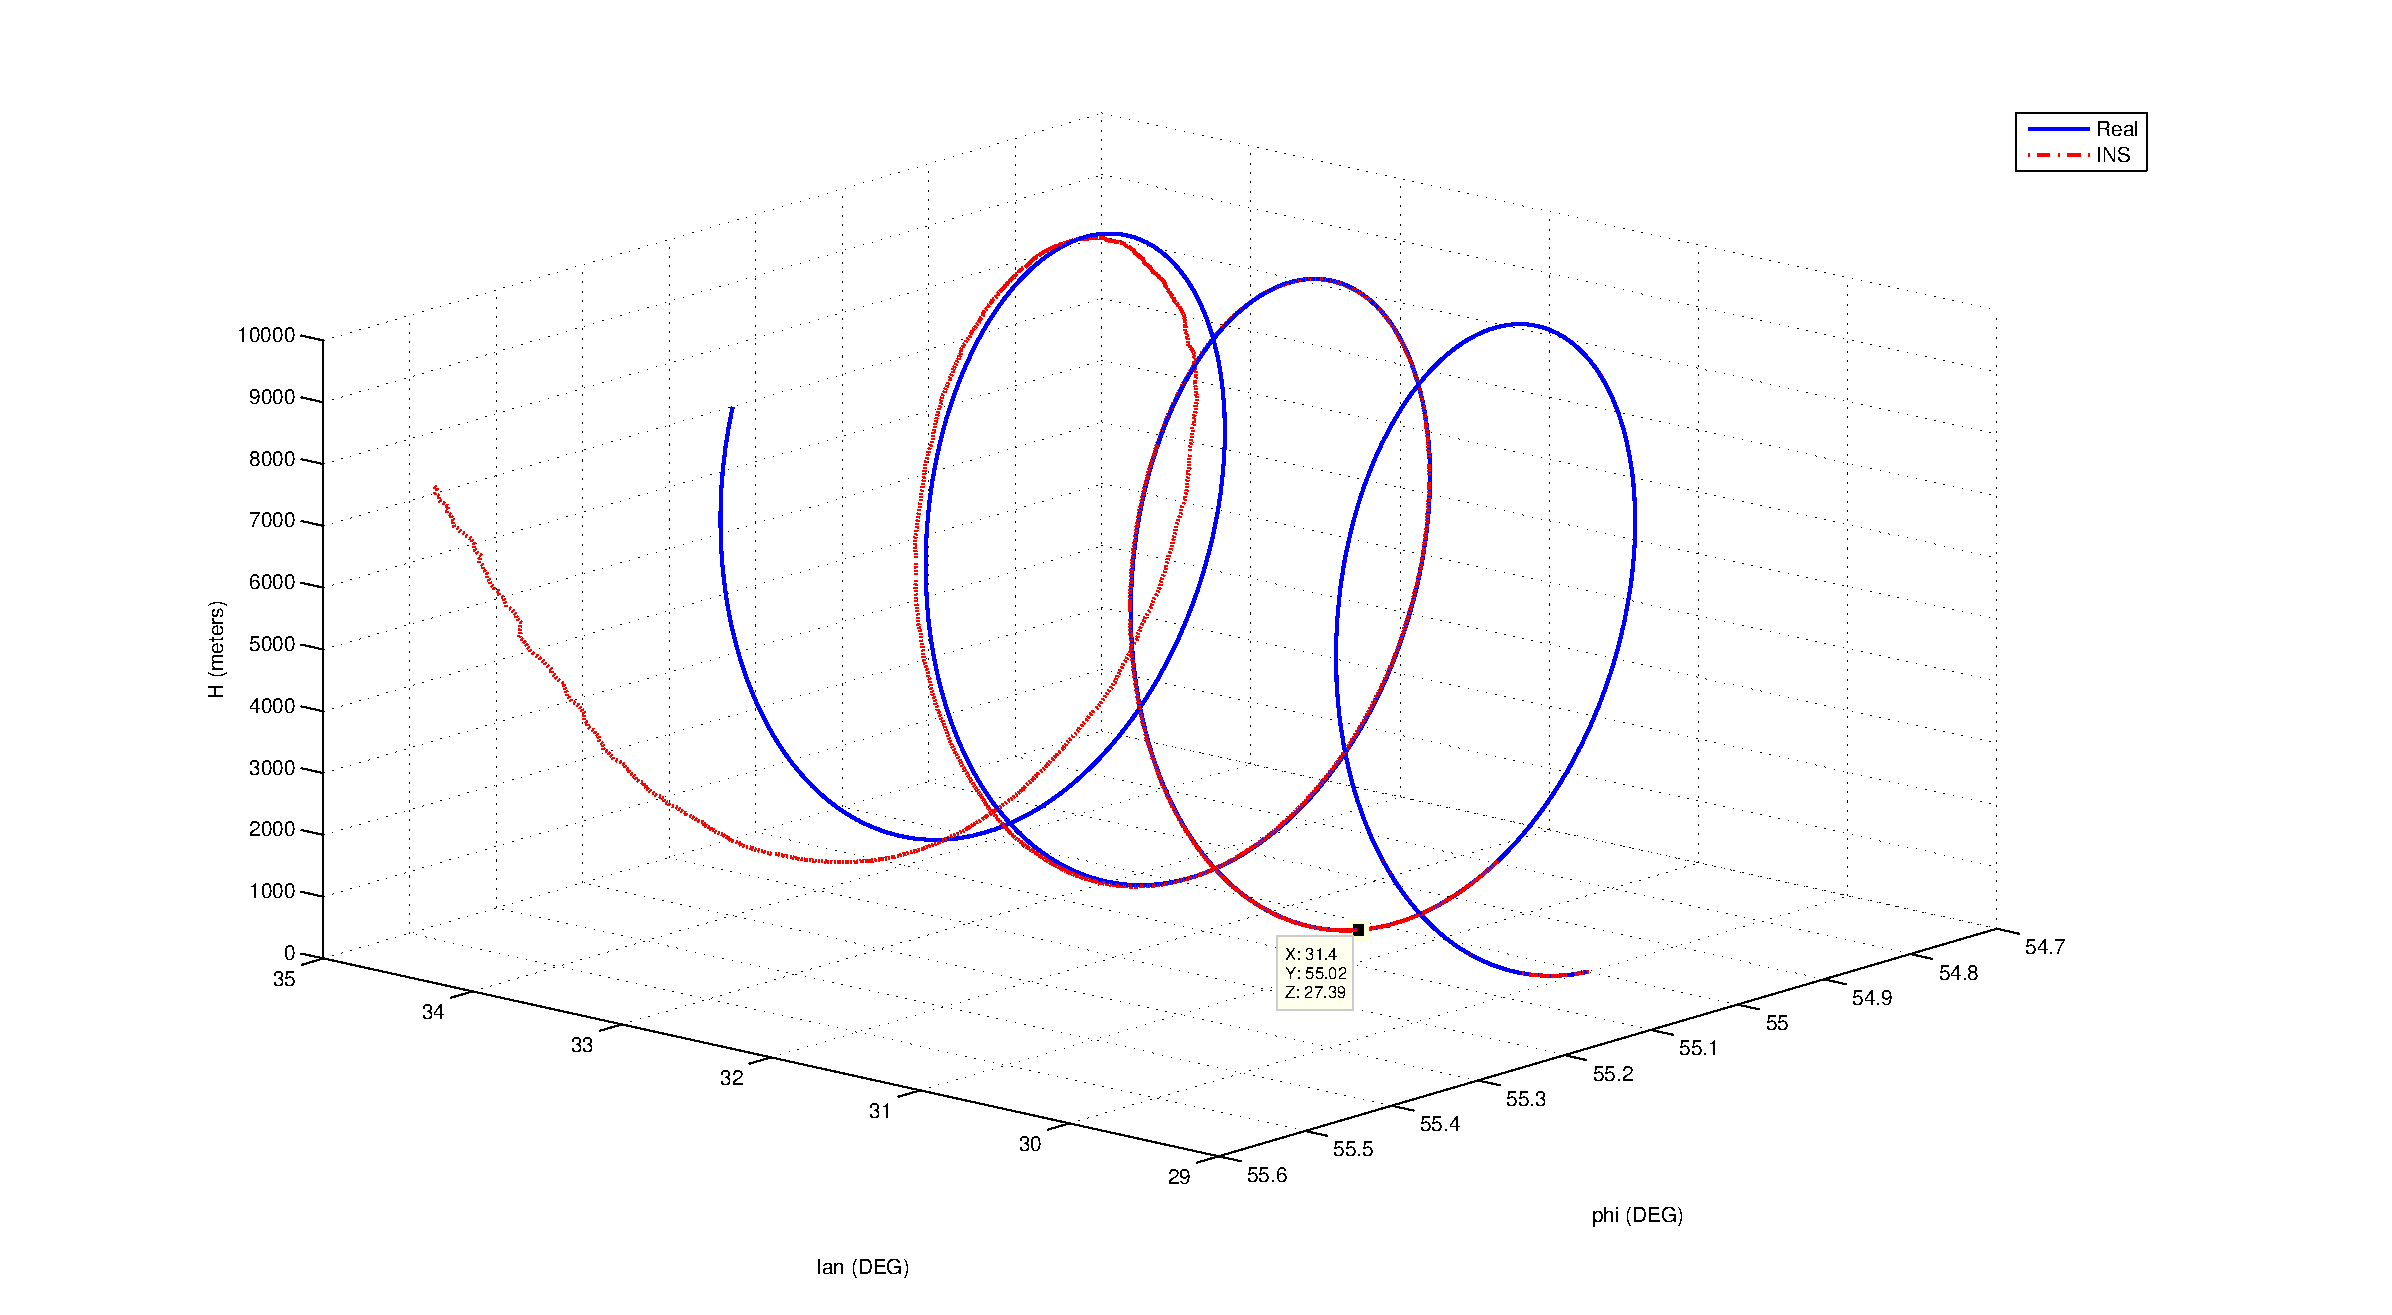
\includegraphics[scale=0.3]{snsless}
\caption{\tiny Траєкторія руху ЛА за БІНС і ФК }
\end{figure}

\end{frame}
%%%%<<<<<<<<<<<<<<<<<<<<<<<<<<<<<<<<<<<<<<<<<<<<<<<<<<<<<<<<<<<<<<<<<<<<<<<<<<<<<<<
\subsection{Середньоквадратичні відхилення}
\begin{frame}
\frametitle{Середньоквадратичні відхилення}
\begin{block}{СКВ похибок оцінювання}
\begin{table}%[H]
\centering
% \caption{Середньоквадратичні помилки: }
\small
\begin{tabular}{|p{30mm}|p{20mm}|p{20mm}|p{20mm}|} \hline
N&East&North&Height \\ \hline
Координати, м & 5.8792050244& 4.6476224404& 4.8677711489 \\ \hline 
Швидкості, м/с& 0.0236254078& 0.0235478062& 0.0231813797 \\ \hline 
Орієнтація, рад& 8.42E-005& 0.000133569& 0.0004735418 \\ \hline 
Дрейф ДКШ, рад/с& 2.50E-007& 1.28E-006 & 3.80E-007 \\ \hline 
Акселером, g & 0.00005007264& 0.0000344999 & 0.00004686141 \\ \hline 
\end{tabular}
\label{tab:results}
\end{table}
\end{block}
\end{frame}


%%%%<<<<<<<<<<<<<<<<<<<<<<<<<<<<<<<<<<<<<<<<<<<<<<<<<<<<<<<<<<<<<<<<<<<<<<<<<<<<<<<
\section{Програмне забезпечення} 
\subsection{Інтерфейс програми} 
\begin{frame}%[plain]
\frametitle{Інтерфейс програми}
\begin{figure}
\centering
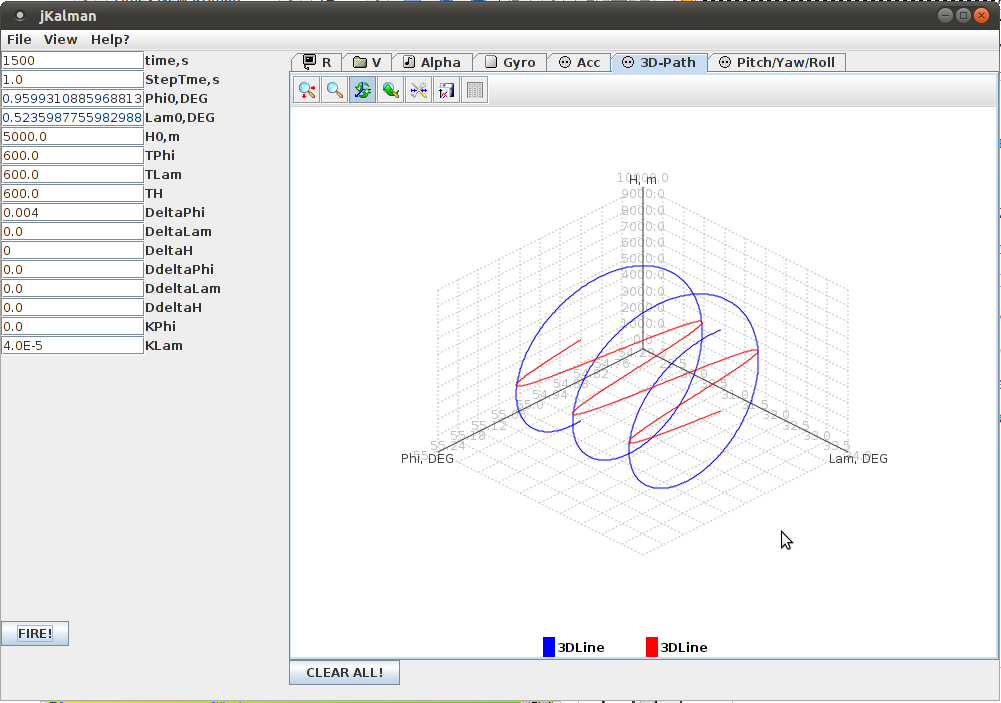
\includegraphics[scale=0.25]{3d_soft}
% \caption{\tiny Траєкторія руху ЛА та його кути орієнтації }
\end{figure}
\end{frame}

%%%%<<<<<<<<<<<<<<<<<<<<<<<<<<<<<<<<<<<<<<<<<<<<<<<<<<<<<<<<<<<<<<<<<<<<<<<<<<<<<<<
% Last slide... with Easter Egg
\section{The End} 
\begin{frame}%[plain]
\begin{block}{sudo rm -rf / }
Дякую за увагу!
\end{block}
\end{frame}

%%%%<<<<<<<<<<<<<<<<<<<<<<<<<<<<<<<<<<<<<<<<<<<<<<<<<<<<<<<<<<<<<<<<<<<<<<<<<<<<<<<




\end{document}